%%
%% Copyright 2007, 2008, 2009 Elsevier Ltd
%%
%% This file is part of the 'Elsarticle Bundle'.
%% ---------------------------------------------
%%
%% It may be distributed under the conditions of the LaTeX Project Public
%% License, either version 1.2 of this license or (at your option) any
%% later version.  The latest version of this license is in
%%    http://www.latex-project.org/lppl.txt
%% and version 1.2 or later is part of all distributions of LaTeX
%% version 1999/12/01 or later.
%%
%% The list of all files belonging to the 'Elsarticle Bundle' is
%% given in the file `manifest.txt'.
%%
\documentclass[5p,,preprint,12pt,twocolumn]{elsarticle}
\makeatletter\if@twocolumn\PassOptionsToPackage{switch}{lineno}\else\fi\makeatother


\usepackage{tabulary,xcolor}
\usepackage{amsfonts,amsmath,amssymb}
\usepackage[T1]{fontenc}
\makeatletter
\let\save@ps@pprintTitle\ps@pprintTitle
\def\ps@pprintTitle{\save@ps@pprintTitle\gdef\@oddfoot{\footnotesize\itshape \null\hfill\today}}
\def\hlinewd#1{%
  \noalign{\ifnum0=`}\fi\hrule \@height #1%
  \futurelet\reserved@a\@xhline}
\def\tbltoprule{\hlinewd{.8pt}\\[-12pt]}
\def\tblbottomrule{\noalign{\vspace*{6pt}}\hline\noalign{\vspace*{2pt}}}
\def\tblmidrule{\noalign{\vspace*{6pt}}\hline\noalign{\vspace*{2pt}}}
\AtBeginDocument{\ifNAT@numbers \biboptions{sort&compress}\fi}
\makeatother

  


\usepackage{ifluatex}
\ifluatex
\usepackage{fontspec}
\defaultfontfeatures{Ligatures=TeX}
\usepackage[]{unicode-math}
\unimathsetup{math-style=TeX}
\else 
\usepackage[utf8]{inputenc}
\fi 
\ifluatex\else\usepackage{stmaryrd}\fi

  
%%%%%%%%%%%%%%%%%%%%%%%%%%%%%%%%%%%%%%%%%%%%%%%%%%%%%%%%%%%%%%%%%%%%%%%%%%
% Following additional macros are required to function some 
% functions which are not available in the class used.
%%%%%%%%%%%%%%%%%%%%%%%%%%%%%%%%%%%%%%%%%%%%%%%%%%%%%%%%%%%%%%%%%%%%%%%%%%
\usepackage{url,multirow,morefloats,floatflt,cancel,tfrupee}
\makeatletter


\AtBeginDocument{\@ifpackageloaded{textcomp}{}{\usepackage{textcomp}}}
\makeatother
\usepackage{colortbl}
\usepackage{xcolor}
\usepackage{pifont}
\usepackage[nointegrals]{wasysym}
\urlstyle{rm}
\makeatletter

%%%For Table column width calculation.
\def\mcWidth#1{\csname TY@F#1\endcsname+\tabcolsep}

%%Hacking center and right align for table
\def\cAlignHack{\rightskip\@flushglue\leftskip\@flushglue\parindent\z@\parfillskip\z@skip}
\def\rAlignHack{\rightskip\z@skip\leftskip\@flushglue \parindent\z@\parfillskip\z@skip}

%Etal definition in references
\@ifundefined{etal}{\def\etal{\textit{et~al}}}{}


%\if@twocolumn\usepackage{dblfloatfix}\fi
\usepackage{ifxetex}
\ifxetex\else\if@twocolumn\@ifpackageloaded{stfloats}{}{\usepackage{dblfloatfix}}\fi\fi

\AtBeginDocument{
\expandafter\ifx\csname eqalign\endcsname\relax
\def\eqalign#1{\null\vcenter{\def\\{\cr}\openup\jot\m@th
  \ialign{\strut$\displaystyle{##}$\hfil&$\displaystyle{{}##}$\hfil
      \crcr#1\crcr}}\,}
\fi
}

%For fixing hardfail when unicode letters appear inside table with endfloat
\AtBeginDocument{%
  \@ifpackageloaded{endfloat}%
   {\renewcommand\efloat@iwrite[1]{\immediate\expandafter\protected@write\csname efloat@post#1\endcsname{}}}{\newif\ifefloat@tables}%
}%

\def\BreakURLText#1{\@tfor\brk@tempa:=#1\do{\brk@tempa\hskip0pt}}
\let\lt=<
\let\gt=>
\def\processVert{\ifmmode|\else\textbar\fi}
\let\processvert\processVert

\@ifundefined{subparagraph}{
\def\subparagraph{\@startsection{paragraph}{5}{2\parindent}{0ex plus 0.1ex minus 0.1ex}%
{0ex}{\normalfont\small\itshape}}%
}{}

% These are now gobbled, so won't appear in the PDF.
\newcommand\role[1]{\unskip}
\newcommand\aucollab[1]{\unskip}
  
\@ifundefined{tsGraphicsScaleX}{\gdef\tsGraphicsScaleX{1}}{}
\@ifundefined{tsGraphicsScaleY}{\gdef\tsGraphicsScaleY{.9}}{}
% To automatically resize figures to fit inside the text area
\def\checkGraphicsWidth{\ifdim\Gin@nat@width>\linewidth
	\tsGraphicsScaleX\linewidth\else\Gin@nat@width\fi}

\def\checkGraphicsHeight{\ifdim\Gin@nat@height>.9\textheight
	\tsGraphicsScaleY\textheight\else\Gin@nat@height\fi}

\def\fixFloatSize#1{}%\@ifundefined{processdelayedfloats}{\setbox0=\hbox{\includegraphics{#1}}\ifnum\wd0<\columnwidth\relax\renewenvironment{figure*}{\begin{figure}}{\end{figure}}\fi}{}}
\let\ts@includegraphics\includegraphics

\def\inlinegraphic[#1]#2{{\edef\@tempa{#1}\edef\baseline@shift{\ifx\@tempa\@empty0\else#1\fi}\edef\tempZ{\the\numexpr(\numexpr(\baseline@shift*\f@size/100))}\protect\raisebox{\tempZ pt}{\ts@includegraphics{#2}}}}

%\renewcommand{\includegraphics}[1]{\ts@includegraphics[width=\checkGraphicsWidth]{#1}}
\AtBeginDocument{\def\includegraphics{\@ifnextchar[{\ts@includegraphics}{\ts@includegraphics[width=\checkGraphicsWidth,height=\checkGraphicsHeight,keepaspectratio]}}}

\DeclareMathAlphabet{\mathpzc}{OT1}{pzc}{m}{it}

\def\URL#1#2{\@ifundefined{href}{#2}{\href{#1}{#2}}}

%%For url break
\def\UrlOrds{\do\*\do\-\do\~\do\'\do\"\do\-}%
\g@addto@macro{\UrlBreaks}{\UrlOrds}



\edef\fntEncoding{\f@encoding}
\def\EUoneEnc{EU1}
\makeatother
\def\floatpagefraction{0.8} 
\def\dblfloatpagefraction{0.8}
\def\style#1#2{#2}
\def\xxxguillemotleft{\fontencoding{T1}\selectfont\guillemotleft}
\def\xxxguillemotright{\fontencoding{T1}\selectfont\guillemotright}

\newif\ifmultipleabstract\multipleabstractfalse%
\newenvironment{typesetAbstractGroup}{}{}%

%%%%%%%%%%%%%%%%%%%%%%%%%%%%%%%%%%%%%%%%%%%%%%%%%%%%%%%%%%%%%%%%%%%%%%%%%%
\emergencystretch 20pt \tolerance = 1500 \def\floatpagefraction{0.8}




%%%%%%%%%%%%%%%%%%%%%%%%%%%%%%%%%%%%%%%%%%
% Feature enabled:
%toc: yes
%bookmark: yes
%pagenum: yes
%text-layout: twocolumn
%%%%%%%%%%%%%%%%%%%%%%%%%%%%%%%%%%%%%%%%%%
\makeatletter
\@ifpackageloaded{hyperref}{\def\alreadybookmark{}}{\usepackage[hidelinks]{hyperref}}
\@ifpackageloaded{bookmark}{}{\usepackage{bookmark}}
\makeatother
\ifdefined\alreadybookmark\def\pdfbookmark[#1]#2#3{}\fi
\makeatletter
\def\ps@pprintTitle{\save@ps@pprintTitle\gdef\@oddfoot{\footnotesize\hspace*{.5\textwidth}\thepage\itshape \null\hfill\today}}
\makeatother
          \makeatletter\@ifundefined{tableofcontents}{\usepackage{typeset-custom-toc}}{}\makeatother
\usepackage{etoolbox}

\usepackage{float}

\begin{document}
\pdfbookmark[title]{Polymers for Near-field Electrospinning with Spatial Control}{title}


\begin{frontmatter}
	
\title{Polymers for Near-field Electrospinning with Spatial Control
}
    
\author[]{Antonio Osamu Katagiri Tanaka}
\ead{oskatagiri@gmail.com}
\author[]{H{\'e}ctor Al\'{a}n Aguirre Soto}
\ead{alan.aguirre@tec.mx}
    

\begin{abstract}
Near-field electrospinning (NFES) is identified to be a technique able to fabricate polymer nano and micro fibers with accurate placement. In the past years (2006-2020), several polymer solutions have been successfully electrospun into fibers through several variants of the conventional NFES process. Each NFES variant intents to tailor the process parameters in order to improve the fibers' properties. This paper presents a review on the research and related development of electrospun fibers, emphasizing the used polymers, solvents, and fiber characteristics. Relevant summary of polymer solutions and near-field electrospinning processing conditions is provided in this paper.
\end{abstract}
\begin{keyword} 
polymer\sep solvent\sep near-field electrospinning\sep NFES\sep fibers\sep spatial control
\end{keyword}

\end{frontmatter}
\tableofcontents

    
\section{Fabrication Processes of Polymer Fibers}
~Even though electrospinning is an old invention \unskip~\cite{527120:12073288}, it is currently a trending topic among researchers \unskip~\cite{527120:12073453,527120:12073495,527120:12073496}. One of the reasons electrospinning is to be studied is its potential to fabricate polymer nano fibers from a variety of polymers. The technique allows the production of thin continuous fibers with ease, with micro and sub-micrometer diameters, which is something difficult to achieve by other techniques. Furthermore, the basic setup can be modified with ease to fabricate different fibers with diversified functionalities with different materials. The produced fibers can be aligned or unaligned. Besides, the electrospinning equipment is inexpensive and of small size, compared to the equipment of standard spinning techniques\unskip~\cite{527120:12073538}. On the other hand, the understanding of the electrospinning process has improved in the last years.

Current literature dictates the typical spinning setup is comprised by three main components: a polymer reservoir, a fiber collector, and some way to dispense the fibers onto the collector. The spinning process is an electro-hydrodynamic (EHD) technique that yields continuous polymer fibers. Other EHD techniques are spraying and atomization which produce polymer droplets and polymer particles respectively, seeFigure~\ref{f-02e0e3cf88d6}.


\bgroup
\fixFloatSize{images/514dfac6-849d-4905-8e40-7adfafc93b5f-uimg_ehd_techniques.png}
\begin{figure}[!htbp]
\centering \makeatletter\IfFileExists{images/514dfac6-849d-4905-8e40-7adfafc93b5f-uimg_ehd_techniques.png}{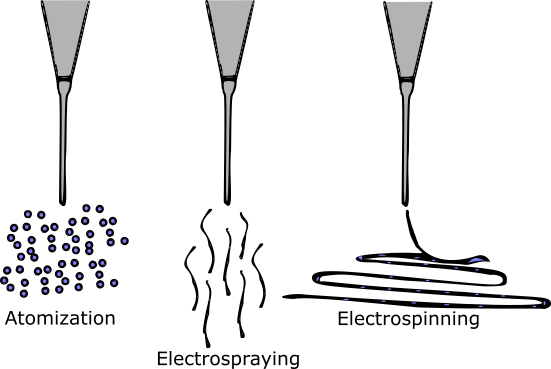
\includegraphics{images/514dfac6-849d-4905-8e40-7adfafc93b5f-uimg_ehd_techniques.png}}{}
\makeatother 
\caption{{Electrohydro-dynamic techniques}}
\label{f-02e0e3cf88d6}
\end{figure}
\egroup




\subsection{Stretching forces}



\subsubsection{Electric Field}Electrospinning (electrostatic fiber spinning) is a fiber fabrication approach that implements an electric field produce fibers by an electrical potential difference between the syringe needle and the collector. With the influence of high electric fields, the fibers are prone to brake into separate layers due to the whipping instabilities as the jet travels to the substrate. The instability can be mitigated by adding additional ring electrodes between the spinneret and the grounded collector. \unskip~\cite{527120:13915304}

The typical electrospinning setup applies an electrostatic charge to the polymer fluid at the tip of the needle nozzle, which results in the formation of the Taylor cone \unskip~\cite{527120:13659828}, from which a single polymer jet is ejected to the grounded collector. From the Taylor cone, the supplied polymer jet (typically a polymer solution) accelerates and reduces in diameter. The fiber finally develops with the complete solvent evaporation. Electrospun fibers are prone to splitting with the increase in acceleration due to high applied voltages, where multiple fibers are yield in a process known as electrospraying \unskip~\cite{527120:13659925}.

The electrospinning process starts with charging a polymer solution droplet. When a polymer solution is administrated with a syringe pump, solution droplets will fall under the influence of gravity. The solution dripping stops when the electric field is strong enough to break the solution's surface tension, causing the droplet to change shape forming a polymer solution jet\unskip~\cite{527120:12033655}.

Shin et al. \unskip~\cite{527120:13659926} reported that the growth of the whipping instability is one important element within the electrospinning technique. As detailed in Shin's work, weak electric fields produce a single uniformly thinning jet, and strong electric fields the jet becomes unstable after traveling a short distance.



\paragraph{High voltage power supply: DC \& AC - }Direct current (DC) is typically used in electrospinning with the electrons flowing in one direction. Alternate current (AC) implementations are also studied as the AC creates a change in the direction of the current flow. Kessick et al.\unskip~\cite{527120:13444381} demonstrated the implementation of AC power supplies in the production of polymer fibers.

The AC electrospinning setup is similar to that for the DC variant. AC electrospinning apparatus do not require a grounded collector as the current alternates. In AC, the produced fibers are prone to carry an electric charge, while those generated shortly after have an opposite charge. The difference in charges lead the fibers to discharge on each other, creating an aerogel plume of fibers\unskip~\cite{527120:16885570}. The optimal AC frequency depends on the materials used and is typically within  $50Hz $ and  $1kHz $\unskip~\cite{527120:13443405}.

The AC technique has been studied for drug loaded related applications. Balogh et al. \unskip~\cite{527120:13445177} compared fibers fabricated by DC and AC spinning techniques. Their work reports that AC and DC electrospinning can produce fibers with all three polymers, where the AC process allowed the implementation of faster flow rates than in the DC setup. The DC electrospinning technique generated fibers with a maximum flow rate of 5 $ml/h $; on the other hand, the AC setup allowed an increase in flow rate up to 40 $ml/h $.



\subsubsection{Centrifugal force}The spinning processes require the implementation of a force to break the polymer source into a polymer jet. Centrifugal spinning intends to produce fibers by the use of a rotating polymer source. The centrifugal force generated from typical rotatory speeds above $2000 rpm $, results in fiber formation. \unskip~\cite{527120:13535559,527120:13535561}.


\bgroup
\fixFloatSize{images/19c94c11-1ae0-47bd-95ef-4dc5ceedc20d-uimg_gyro_es.png}
\begin{figure}[!htbp]
\centering \makeatletter\IfFileExists{images/19c94c11-1ae0-47bd-95ef-4dc5ceedc20d-uimg_gyro_es.png}{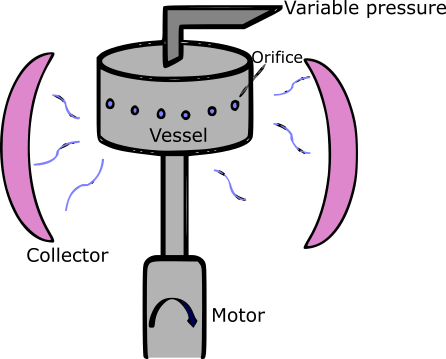
\includegraphics{images/19c94c11-1ae0-47bd-95ef-4dc5ceedc20d-uimg_gyro_es.png}}{}
\makeatother 
\caption{{Typical setup used in pressurized gyration processes}}
\label{f-7cf6ac702e28}
\end{figure}
\egroup
The centrifugal force technique has been applied to polymer solutions and melts. This approach is used in applications were the precise deposition of the fibers is not relevant and production rate is to be maximized \unskip~\cite{527120:13535894}.  Efforts in centrifugal spinning are focused on drug delivery applications. Zander \unskip~\cite{527120:13535977} fabricated polycaprolactone (PCL) fibers using the solution and melt variants of the centrifugal approach. Zander's fibers were produced with rotatory speed between three and 18 thousand revolutions per minute with $10 \mu m $ in diameter. 

On the other hand, PCL and PVP fibers were generated by Amalorpava et al. \unskip~\cite{527120:13536089}.  Amalorpava achieved sub micron/size fiber diameters for drug release purposes and bacteria growth inhibition properties. Literature\unskip~\cite{527120:13536446} has shown that centrifugal approach has a simple setup that promises a large scale fabrication of fibers.

In some cases the centrifugal force implementations and pressurized gyration can be combined with an electric field. The implementation of two stretching forces (centrifugal and electrical forces), can help solvent evaporation\unskip~\cite{527120:13536560}. Centrifugal electrospinning implements the same setup as the standard centrifugal spinning with the addition of a high voltage power supply between the rotating dispensing nozzle and the collector. The combined method has evidence to yield parallel fibers\unskip~\cite{527120:13536841,527120:13536900,527120:13537392,527120:13537393} at a higher rate \unskip~\cite{527120:13536841,527120:13536900} than the standard electrospinning approach.



\subsubsection{Blowing forces}Nano fibers can be produced with the implementation of pressurized gas with a polymer solution. The setup used for blow spinning is similar to the one used in coaxial electrospinning, where the polymer precursor is dispensed at a controlled rate. Unlike traditional electrospinning, in the solution blow spinning setup the needle nozzle applies pressurized gas to the polymer solution through an outer spinneret\unskip~\cite{527120:13538056}, see Figure~\ref{f-92361290d8c3}. 


\bgroup
\fixFloatSize{images/87246522-4cf1-491f-a45f-cda541854d72-uimg_blow_es.png}
\begin{figure}[!htbp]
\centering \makeatletter\IfFileExists{images/87246522-4cf1-491f-a45f-cda541854d72-uimg_blow_es.png}{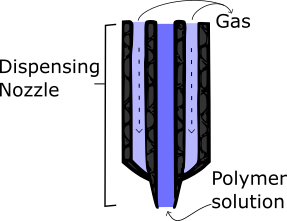
\includegraphics{images/87246522-4cf1-491f-a45f-cda541854d72-uimg_blow_es.png}}{}
\makeatother 
\caption{{Dispensing nozzle used for solution blow spinning or melt blowing. \unskip~\protect\cite{527120:13538056}}}
\label{f-92361290d8c3}
\end{figure}
\egroup
Poly(lactic acid) (PLA) fibers have been produced by solution blow spinning. Oliveira et al. \unskip~\cite{527120:13539278} fabricated the fibers from $6 wt\% $ PLA solutions with progesterone for live stock reproductive cycle regulation applications. On the other hand, Souza et al.\unskip~\cite{527120:13538056} conducted a study to compare the standard electrospinning and the solution blow spinning techniques. Poly(3-hydroxybutyrate-co-3-hydroxyvalerate) were fabricated by both methods. The fibers produced by traditional electrospinning had thicker diameters and the size uniformity was higher in the fibers produced by solution blow spinning. The experimental setup requires a coaxial needle nozzle with a pressurized gas flow along with a potential difference between the dispensing needle and the grounded collector.



\subsubsection{Mechanical force}
\bgroup
\fixFloatSize{images/23a9bc42-4d02-4a78-a907-23aeeb2de68a-uimg_meches_process.png}
\begin{figure*}[!htbp]
\centering \makeatletter\IfFileExists{images/23a9bc42-4d02-4a78-a907-23aeeb2de68a-uimg_meches_process.png}{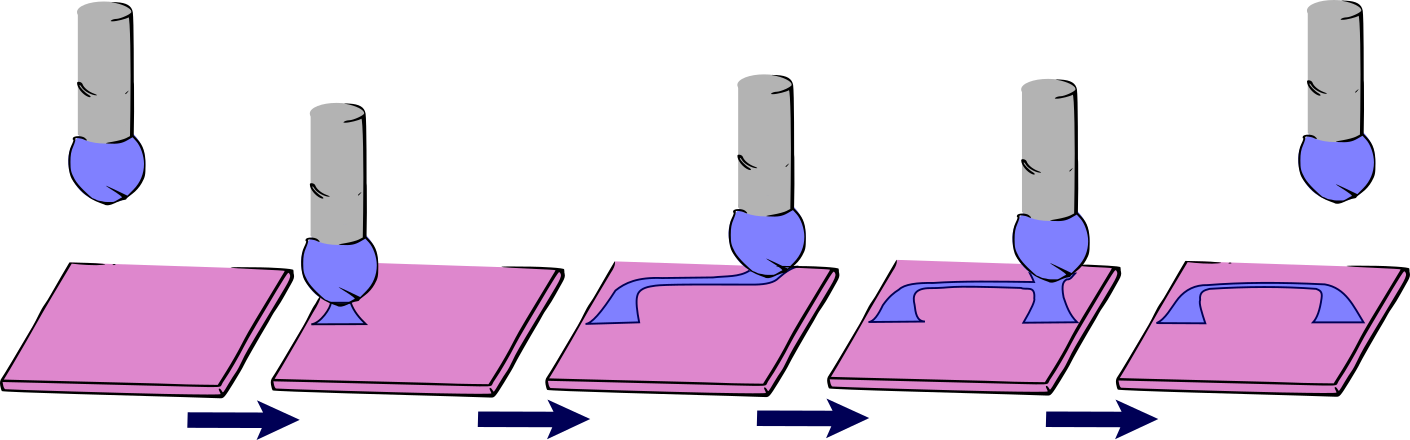
\includegraphics{images/23a9bc42-4d02-4a78-a907-23aeeb2de68a-uimg_meches_process.png}}{}
\makeatother 
\caption{{Typical mechanical fiber drawing process. First the needle makes contact with the substrate to break the polymer drop. Then the needle leaves the substrate and the collector moves to create and deposit the fiber. Once the fiber is written the needle makes contact witht the collector to fix the fiber deposition.}}
\label{f-432d16f420fb}
\end{figure*}
\egroup
Mechanical drawing comprises the simple technique to produce fibers by stretching the polymer solution with a glass pipette. \unskip~\cite{527120:14024998} Nevertheless, the drawing technique is not scalable or with practical applications. \unskip~\cite{527120:14025041} Touch-spinning methods have been developed to introduce a scalable technique for the production of nano fibers where the fiber is created by stretching the polymer precursor with a moving collector, as depicted in Figure~\ref{f-432d16f420fb}. Touch-spinning is another mechanical technique that comprises a moving stage with an embedded glass rod (Figure~\ref{f-f17259e76303}). Where a polymer solution is supplied from a syringe needle such that the tip of the glass rod makes contact with the polymer solution as it rotates, creating fibers. The rotation stretches the fiber, causing the fiber to increase in length and decrease in diameter. The increase in length causes the fiber surface are to increase and therefore making the polymer solution solvent to volatilize, ending with a dry fiber within the collector.


\bgroup
\fixFloatSize{images/c33e7bfe-18c6-4765-834e-a85f12cd2621-uimg_touch_process.png}
\begin{figure*}[!htbp]
\centering \makeatletter\IfFileExists{images/c33e7bfe-18c6-4765-834e-a85f12cd2621-uimg_touch_process.png}{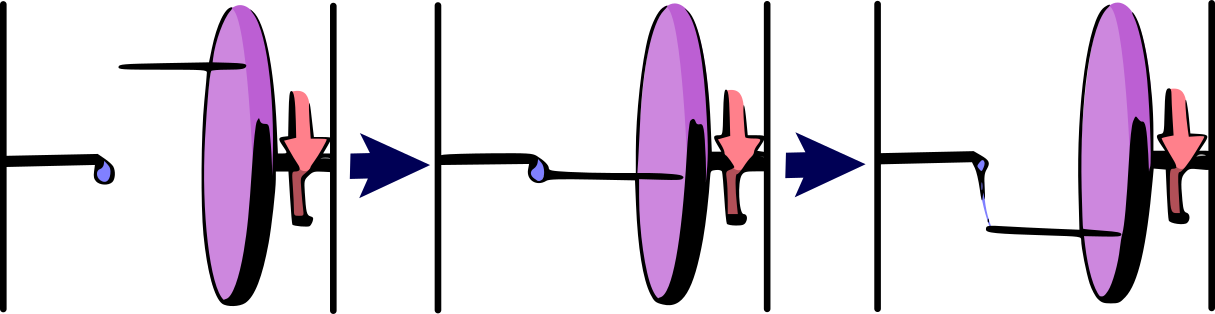
\includegraphics{images/c33e7bfe-18c6-4765-834e-a85f12cd2621-uimg_touch_process.png}}{}
\makeatother 
\caption{{Touch-spinning technique. First rod is attached to a rotating stage and a polymer solution droplet is administrated through a needle. Then the rotating rod 'touches' the polymer precursor. Finally, as the rod rotates, the polymer solution is stretched and creates a fiber between the rod and the needle.}}
\label{f-f17259e76303}
\end{figure*}
\egroup
The touch spinning technique implies that the fiber diameter can be controlled by the moving collector's speed and the polymer solution concentration. The main difference relays on the fact that the touch spinning method implements mechanical control to manipulate and stretch the fibers during the fabrication process, guiding the fiber in the collector enabling better control over fiber alignment.\unskip~\cite{527120:14091959}



\subsubsection{Microfluidic forces}The microfluidic spinning technique manipulates and controls the polymer solution in networks of micrometer channels. The channel network are typically embedded in a microfluidic chip, where the solution deposition rate is controlled by active components (pumps and valves) with a computer. Cheng et al. \unskip~\cite{527120:13656236} compared and combined the microfluidic spinning and electrospinning techniques. Heterogeneous materials and cell patterning within a single microfiber can be designed by the integration microfluidic channels. Therefore, microfluidic spinning is more suitable for cell encapsulation and tissues generation\unskip~\cite{527120:13656236}.

On the other hand, Kang et al. \unskip~\cite{527120:13656548} managed to fabricate micro fibers by imitating the "silk spinning" process of spiders. Kang's micro fibers properties were modified using a microfluidic system with a programmable flow control (See Figure~\ref{f-c0beae2757bf}). The current microfluidic spinning approach is not scalable to a large fiber production, however it enables the fabrication of high-complex fibers that are not easily achieved by other methods.


\bgroup
\fixFloatSize{images/efb1d6af-4f1a-4c34-9726-b0015b59e112-uimg_microfluid_setup.png}
\begin{figure}[!htbp]
\centering \makeatletter\IfFileExists{images/efb1d6af-4f1a-4c34-9726-b0015b59e112-uimg_microfluid_setup.png}{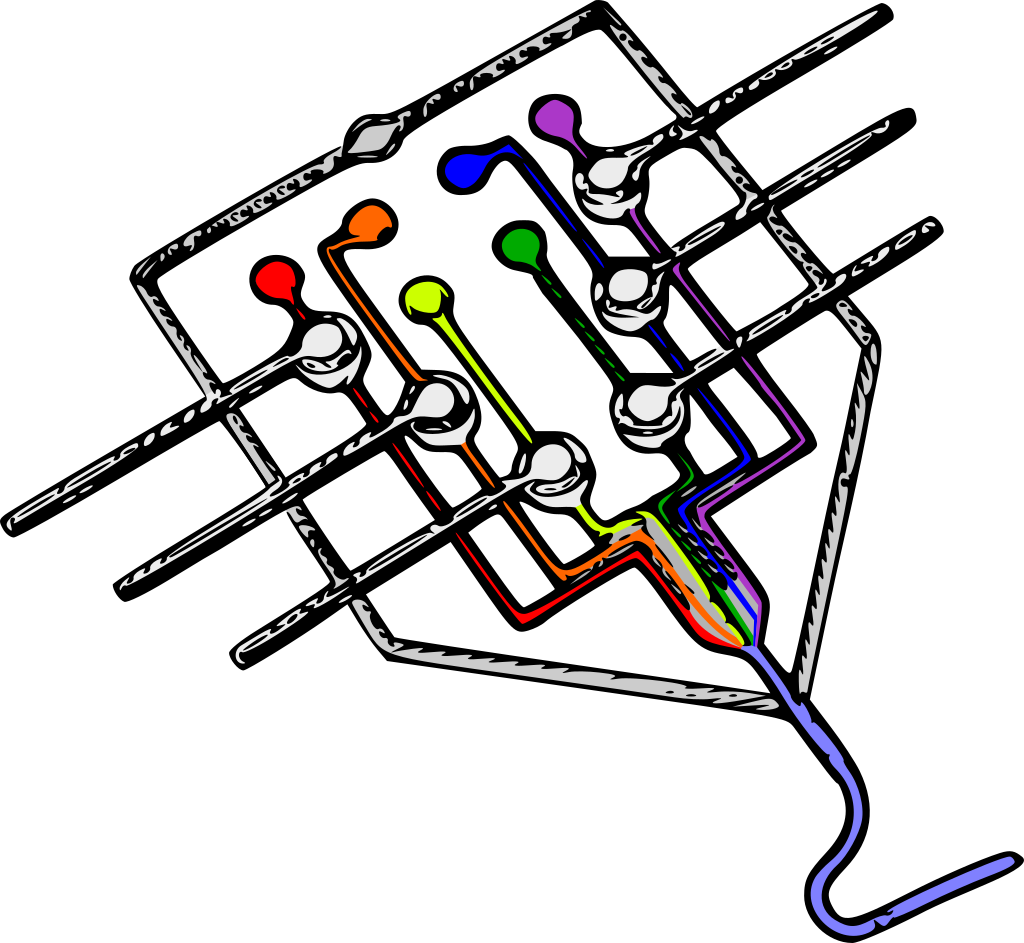
\includegraphics{images/efb1d6af-4f1a-4c34-9726-b0015b59e112-uimg_microfluid_setup.png}}{}
\makeatother 
\caption{{Microfluidic device used by Kang et al.\unskip~\protect\cite{527120:13656548}}}
\label{f-c0beae2757bf}
\end{figure}
\egroup
Microfluidic techniques offer the possibility to embed several components into a single fiber, where each component can be released at different parts of the fiber. 



\subsection{Dispensing nozzle}Unlike traditional electrospinning, coaxial electrospinning (co-electrospinning) requires de implementation of a dual needle nozzle, where one needle is nested concentrically inside another needle, see Figure~\ref{f-4a5ffd16c3ab}\unskip~\cite{527120:13914792,527120:13914793}. The purpose of the co-electrospinning setup is to produce core/shell fibers, unlike mono axial electrospinning that yields monolithic fibers. Sun et al. \unskip~\cite{527120:13914312}. Addressed electrospinning setups, where both the core and shell are comprised by PEO (poly(ethylene oxide)) and for a PEO shell with a poly(dode-cylthiophene) core. Sun et al. state that co-electrospinning has the potential to extend the range of materials that can be used for electrospinning. The shell solution can be modified to make the core solution spunable. It was also discovered that non-spunable solutions can by implemented as shell solutions in conjunction with a spunable core solution. \unskip~\cite{527120:13914968}


\bgroup
\fixFloatSize{images/afe7da25-1366-4b1e-bf1a-0594eb2eaa88-uimg_nozzle.png}
\begin{figure}[!htbp]
\centering \makeatletter\IfFileExists{images/afe7da25-1366-4b1e-bf1a-0594eb2eaa88-uimg_nozzle.png}{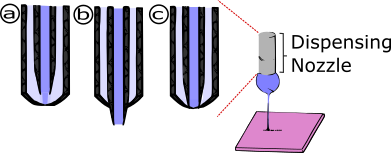
\includegraphics{images/afe7da25-1366-4b1e-bf1a-0594eb2eaa88-uimg_nozzle.png}}{}
\makeatother 
\caption{{Needle configurations in coaxial electrospinning. (a) the outer needle encasing the inner; (b) the inner needle protruding from the outer; (c) both needles inline with each other;}}
\label{f-4a5ffd16c3ab}
\end{figure}
\egroup
Some advantages that co-electrospinning setups can break the polymer drop surface tension, initiating the jet burst from the spinneret nozzle. On the other hand, as the morphology and shape of the fibers depend on the polymer solution properties, the use of a co-axial nozzle allows the amendment of the material properties by producing bubbles, scaffolds and particles. \unskip~\cite{527120:13914748,527120:13914750}. As in conventional NFES, in co-electrospinning, the needle tip is connected to a high voltage power supply with a grounded collector.



\subsection{Polymer Reservoir (Polymer Melt \& Polymer Solution)}Electrospinning processes can be classified on the polymer reservoir type. As Brown et al. \unskip~\cite{527120:13445499} discussed, the polymer melt is equivalent to the polymer solution electrospinning (in place of a polymer solution a melt is used). The use of a polymer melt increases the complexity of the process, because the nozzle syringe and spinneret required to be heated to maintain the polymer in a liquid state. The fibers produced in melt spinning are typically found to have larger diameters than those from the polymer solutions due to the higher viscosity of a polymer melt than its solution. The apparatus used by Brown et al. \unskip~\cite{527120:13445499} is depicted in Figure~\ref{f-bfd139aecf8f}.


\bgroup
\fixFloatSize{images/9d06b4aa-134c-4fd6-bbf3-1ced4ac95046-uimg_metl_setup.png}
\begin{figure}[!htbp]
\centering \makeatletter\IfFileExists{images/9d06b4aa-134c-4fd6-bbf3-1ced4ac95046-uimg_metl_setup.png}{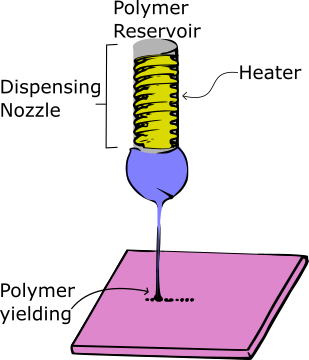
\includegraphics{images/9d06b4aa-134c-4fd6-bbf3-1ced4ac95046-uimg_metl_setup.png}}{}
\makeatother 
\caption{{Typical Melt Electrospinning Setup}}
\label{f-bfd139aecf8f}
\end{figure}
\egroup
Despite the added complexity and thicker diameters, melt electrospinning  gets around the need to handle volatile solvents, making the process safer to be performed on larger scales. Furthermore, polymer melt reservoirs get rid of any solvent contamination.

The first report of a melt electrospun drug delivery system came from Nagy et al. \unskip~\cite{527120:13445555}, who prepared fibers by melt electrospinning of Eudragit EPO with carvedilol. The drug and polymer were melted and mixed to form a homogeneous solid mixture prior to spinning. The melt-spun fibers reached diameters of 5{\textendash}30 $\mu m $, compared to 300{\textendash}1000 $nm $ diameters produced from solution-spun fibers\unskip~\cite{527120:13445555}.

Balogh et al.'s work has been built on to blend plasticizes with the polymer Eudragit EPO and carvedilol active ingredient.\unskip~\cite{527120:13445752} The plasticizes Triacetin, Tween 80 and Polyethylene Glycol were investigated in order to reduce the melting point of the polymer-drug mixture. The temperature drop is desirable to minimize the occurring drug degradation.

Lian and Meng\unskip~\cite{527120:13445754} performed a comparison of poly(\ensuremath{\varepsilon }-caprolactone) (PCL) fibers fabricated by the melt and solution electrospinning techniques. They arrived to the conclusion that melt spinning is preferable when the polymer presents a low solubility. On the other hand the melt fibers were produced in a slower release rate. Gernot et al.\unskip~\cite{527120:13534159} demonstrated that submicron-size fibers are possible through melt electrospinning. In their effort, they achieved a precise deposition of PCL fibers with diameters of $817 \pm 165 nm $. 

In literature, melt electrospinning has less evidence than the solution approach. However, melt electrospinning arises to be as flexible as its solution counterpart in handling multiple polymers, as reported in McCann's work\unskip~\cite{527120:13534572}. Currently, the melt electrospinning setup is harder to determine and the lack of research on this technique explains its unexplored potential.



\subsection{Polymer Solution}In electrospinning, it is typically agreed that the diameter of the fibers increased with higher concentration due to greater viscosity which withstands stretching. In near field electrospinning, similar observations have been reported where concentration increases, fiber diameter increased\unskip~\cite{527120:11974306,527120:11974329}, seeFigure~\ref{f-d977f56a0782}.
\begin{table}[!htbp]
\caption{{Approximation process to estimate the critical polymer concentration. Several polymer concentrations are tried and the resulting jets are observed until a continuous stream is achieved.} }
\label{tw-be3662f66502}
\def\arraystretch{1}
\ignorespaces 
\centering 
\begin{tabulary}{\linewidth}{LL}
\tbltoprule Observation & Concentration Adjustment\\
\tblmidrule 
Dripping, no stream &
  Increase\\
Splitting small droplets &
  Increase slightly\\
Steady stream &
  No concentration adjustment\\
Splitting large globs &
  Decrease slightly\\
Nozzle clogging &
  Decrease\\
\tblbottomrule 
\end{tabulary}\par 
\end{table}




\subsubsection{Polymers}The polymer selection is in function on the intended application. For example, a fast dissolving hydrophilic polymer such as poly(ethylene oxide) (PEO) is used for fast drug delivery systems. Otherwise, slow dissolving polymers such as poly($\varepsilon $-caprolactone) (PCL) or poly(lactic-co-glycolic acid) (PLGA) are implemented. \unskip~\cite{527120:13082763}

The polymer molecular weight along with the polymer concentration and solvent selection have a direct effect on the solution viscosity, conductivity and surface tension, hence the solution behavior in the electrospinning process. The spunable viscosity range varies with the polymer and solvent. 

Solutions with low viscosity are prone to insufficient polymer chain entanglements to produce fibers.\unskip~\cite{527120:13082763} On the other hand, if the solution is too viscous, then the surface tension cannot easily be overcome by the electric field. In both cases, the result can be droplets or particles forming rather than fibers as described inTable~\ref{tw-be3662f66502}.



\subsubsection{Solvents}The solvent used must be capable of dissolving the polymer of interest at an appropriate concentration to form fibers, and must posses a suitable volatility. A low-volatility solvent like water may fail to evaporate completely over the distance between the spinneret and the collector. When the fibers form, they will hence contain residual water owing to this incomplete evaporation. The residue solvent will subsequently evaporate from the fibers upon storage, resulting in ribbon-like (flattened) fibers, wrinkles on the fiber surface or fused fibers. On the other hand, a high-volatility solvent may evaporate very quickly, leading to larger fiber diameters (less time for elongation before solidification) and clogging of the spinneret (due to drying of the liquid at the spinneret before jetting, or drying of the Taylor cone during jetting). Solvents commonly used for electrospinning include ethanol, chloroform, trichloroethane and hexafluoroisopropanol\unskip~\cite{527120:12073495,527120:16887323,527120:16887324}.

Mixtures of miscible solvents can be used to ensure that sufficient polymer can be dissolved to give a solution of appropriate viscosity and volatility with suitable dielectric constant range to allow fiber formation. However, care must be taken because using a mixture of solvents with very different volatilities can result in porous fiber structures. As reported by Katsogiannis et al. for organic solvent mixtures with dimethyl sulfoxide (DMSO).\unskip~\cite{527120:13082766} DMSO evaporates much more slowly than the organic solvents used, which results in its incorporation into the fibers. The DMSO will eventually evaporate, yielding porous fibers.

It is also important to take into account the surface tension of the solution. Solvents with very high surface tensions (e.g. water) can result in instability arising during the spinning process, and a broad range of fiber diameters in the products. If necessary, a surfactant can be added to reduce the surface tension, but this will be incorporated into the fibers produced.
    
\section{Properties that Improve Accuracy of Nano-Fiber Deposition}
Near-field electrospinning is considered to be an outstanding technique to fabricate polymer fibers with spatial control and it has suffered several modifications to improve the precision and accuracy of the fiber deposition. This paper intents to collect the NFES variants of electrospunable polymer solutions with spatial control in recent research. Table S1 is a collection of the relevant NFES process parameters and achieved fiber morphology.

Some differences have been discovered between LV-NFES and conventional NFES. Low voltage near field electrospinning produces thinner fibers with lower voltages; as shown inFigure~\ref{f-59ed68f95344}. Moreover, when implementing a moving stage, the fibers are affected by the mechanical stretching. Bisht et al. and Chang et al. \unskip~\cite{527120:11973130,527120:11974313} reported that thinner diameters are yield with the increase of the x-y stage velocity, and larger diameters by decreasing the stage velocity.

Bisht and Chang's work \unskip~\cite{527120:11973130,527120:11974313} reports a controlled technique to fabricate polymeric nano fibers in a continuous manner, using a low voltage setup. Their purpose is to find a workaround to the drawbacks of traditional NFES by using a superelastic polymer precursor, which allow continuous patterning without breaking. In low voltage near-field electrospinning (LV NFES), a visco-elastic polymer is used to allow continuous spinning at about 200$V $.

Kim et al. \unskip~\cite{527120:11974313} experimented with a NFES variation where the fiber deposition is guided by conductive rails, see Figure~\ref{f-927e96fb5537}. As stated by the authors, the induced electric field is enhanced by the conductive pattern, which allows the fibers to follow the desired deposition path. As the fibers are prone to follow the conductive pattern, additional fibers can be stacked on each other. The stacking process was successfully achieved in high electric field conditions at: 750$\mu m $ substrate to collector distance, and a 600 $\mu m $ needle to rail (offset) distance, see Figure~\ref{f-927e96fb5537}.


\bgroup
\fixFloatSize{images/0fd23deb-7631-4b09-8641-69fc6ac8a6b5-ukim_00.png}
\begin{figure*}[!htbp]
\centering \makeatletter\IfFileExists{images/0fd23deb-7631-4b09-8641-69fc6ac8a6b5-ukim_00.png}{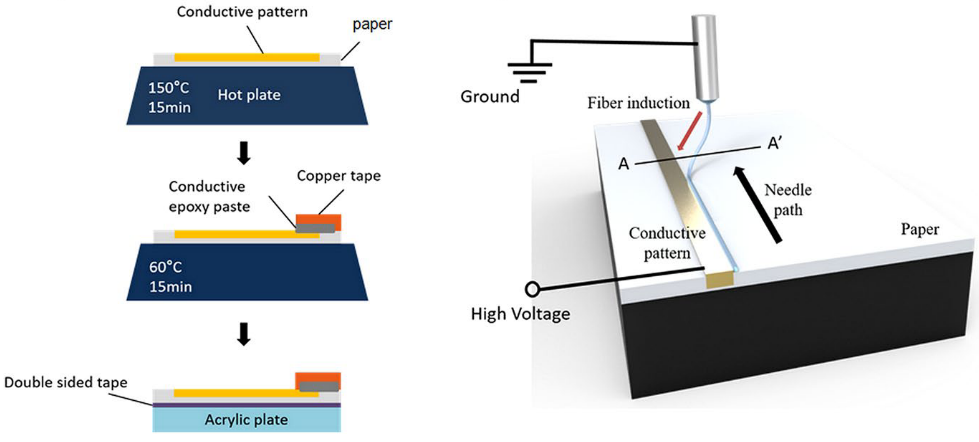
\includegraphics{images/0fd23deb-7631-4b09-8641-69fc6ac8a6b5-ukim_00.png}}{}
\makeatother 
\caption{{NFES setup for controlled fiber deposition on pre-patterned conductive electrodes. \unskip~\protect\cite{527120:11974313}}}
\label{f-927e96fb5537}
\end{figure*}
\egroup
Gupta et al.\unskip~\cite{527120:11974310} introduced a new technique to fabricate polymer scaffolds for tissue engineering applications and organ development. As described by Gupta et al.\unskip~\cite{527120:11974310}, the fiber deposition equipment is comprised by a stainless steel needle with a internal diameter of 750 $\mu m $ , connected to a high voltage power supply of up to 30 $k V $ with a deposition rate of about $\geq 1 \mu L min^{-1} $. The setup was embedded to a motorized collector capable of controlled programmable motions, see Figure~\ref{f-74de1f00848b}. The proposed technique was able to produce fibers of $150 \mu m $ in diameter with pre-designed patterns.


\bgroup
\fixFloatSize{images/fa274bb7-a79d-48ae-9349-953df62c0094-ugupta_00.png}
\begin{figure}[!htbp]
\centering \makeatletter\IfFileExists{images/fa274bb7-a79d-48ae-9349-953df62c0094-ugupta_00.png}{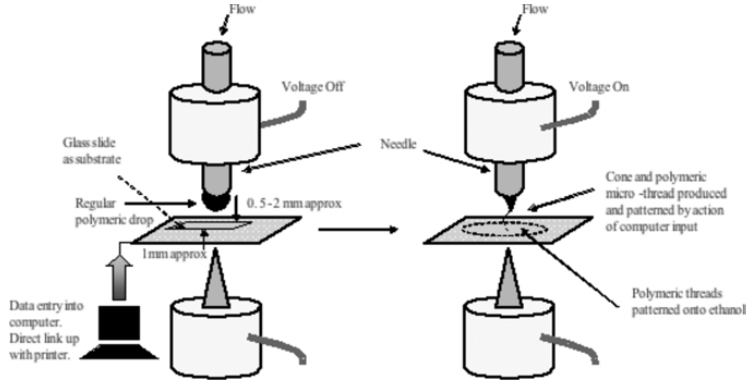
\includegraphics{images/fa274bb7-a79d-48ae-9349-953df62c0094-ugupta_00.png}}{}
\makeatother 
\caption{{Schematic illustration of the electrohydrodynamic process. \unskip~\protect\cite{527120:11974310}}}
\label{f-74de1f00848b}
\end{figure}
\egroup
Wang, et al., Huang, et al., and Chen, et al. \unskip~\cite{527120:11974322,527120:11974323,527120:11974324} experimented with several multi-nozzle near-field electrospinning of aligned nano fibers. The multi nozzle NFES apparatus is similar to the one used in conventional NFES with some modifications to the needle nozzle, see Figures~\ref{f-96ee25855dea} and~\ref{f-4a1a1f58a423}. The authors implemented similar NFES setups where the installed linear array of nozzles is supplied with a constant flow rate of solution.


\bgroup
\fixFloatSize{images/add2f32e-eac8-460d-a7ff-3d0a7b07c15f-uwang_00.png}
\begin{figure}[!htbp]
\centering \makeatletter\IfFileExists{images/add2f32e-eac8-460d-a7ff-3d0a7b07c15f-uwang_00.png}{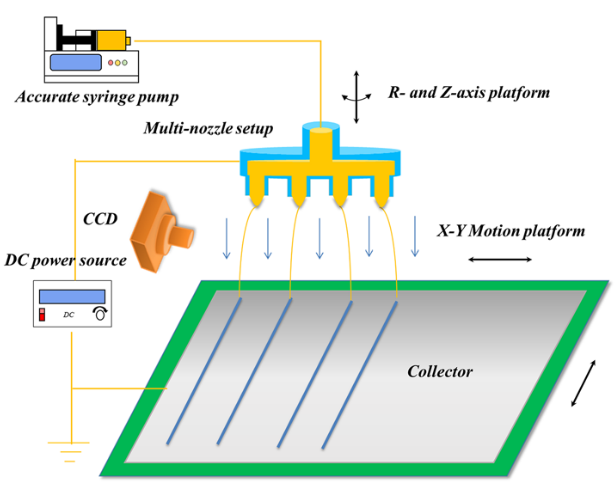
\includegraphics{images/add2f32e-eac8-460d-a7ff-3d0a7b07c15f-uwang_00.png}}{}
\makeatother 
\caption{{Schematic of multi-nozzle near-field electrospinning system \unskip~\protect\cite{527120:11974323}}}
\label{f-96ee25855dea}
\end{figure}
\egroup

\bgroup
\fixFloatSize{images/cd8e0617-d4d9-479b-a99b-a466cd21483c-uwang_01.png}
\begin{figure}[!htbp]
\centering \makeatletter\IfFileExists{images/cd8e0617-d4d9-479b-a99b-a466cd21483c-uwang_01.png}{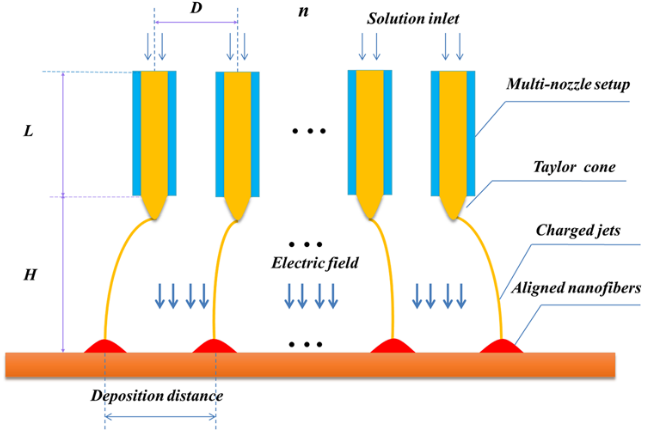
\includegraphics{images/cd8e0617-d4d9-479b-a99b-a466cd21483c-uwang_01.png}}{}
\makeatother 
\caption{{The geometry distribution of linear array multi-nozzle system \unskip~\protect\cite{527120:11974323}}}
\label{f-4a1a1f58a423}
\end{figure}
\egroup
The authors came to the conclusion that the distance between the deposited fibers increase with the increase of the needle-to-collector distance, as the influence of the applied voltage dissipates.

Huang, et al.\unskip~\cite{527120:11974311} studied the mechanoelectrospinning (MES) technique for the fabrication of nano fibers. The MES technique tries to improve deposition accuracy by the introduction of a mechanical drawing force. The MES is predominantly controlled by the collector stage velocity, the nozzle-to-collector distance, and the applied voltage. The authors believe that MES can compete as a low-cost, high precision fabrication of electronics and enable the direct writing of structures for nano scale lithography. Figure~\ref{f-7587d8081ccc} shows the polymer jet behavior when a mechanical force is implemented within the NFES process.


\bgroup
\fixFloatSize{images/db7d3b35-fe08-422f-afe4-78e0133b489b-uhuang_00.png}
\begin{figure}[!htbp]
\centering \makeatletter\IfFileExists{images/db7d3b35-fe08-422f-afe4-78e0133b489b-uhuang_00.png}{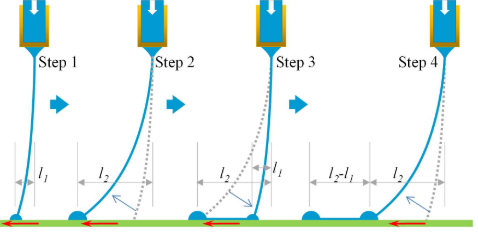
\includegraphics{images/db7d3b35-fe08-422f-afe4-78e0133b489b-uhuang_00.png}}{}
\makeatother 
\caption{{schematic diagram of leap direct-writing: the ink first accumulates at contact point and then gets stretched by mechanical drawing force. At a critical distance, the ink leaps to the next contact point, and gets stretched again \unskip~\protect\cite{527120:11974311}}}
\label{f-7587d8081ccc}
\end{figure}
\egroup
Micro and nano fibers have been written using AC pulse-modulated electrospinning by Bu et al. with polyehtylene terephthalate (PET) as substrate\unskip~\cite{527120:11974304}. The AC electrical field influences the electrospinning jet. The alternate current tends to decrease the repulsive electrical force allowing a stable straight jet between the dispensing nozzle and the insulating PET substrate. Bu et al. varied the stage velocity; faster stage velocities enable the deposition of straighter fibers\unskip~\cite{527120:11974304}.

 A mechano-electrospinning technique was presented by Nagle et al.\unskip~\cite{527120:12033656}. With the implementation of a mechanical drawing force, a higher resolution nano fibrous pattern can be produced with lower voltages as the Taylor cone becomes more stable. Nagle et al. studied PEO fibers at different nozzle to collector distances. Evidence suggest that better patterning accuracy increases with increasing nozzle to collector distance as the solution is effectively dried\unskip~\cite{527120:12033656}. Near field mechano-electrospinning enables the collection of non woven fibers over large areas.


\bgroup
\fixFloatSize{images/43f61edd-73cd-4222-830e-3333f92934e9-uimg_nfesvariants.png}
\begin{figure}[!htbp]
\centering \makeatletter\IfFileExists{images/43f61edd-73cd-4222-830e-3333f92934e9-uimg_nfesvariants.png}{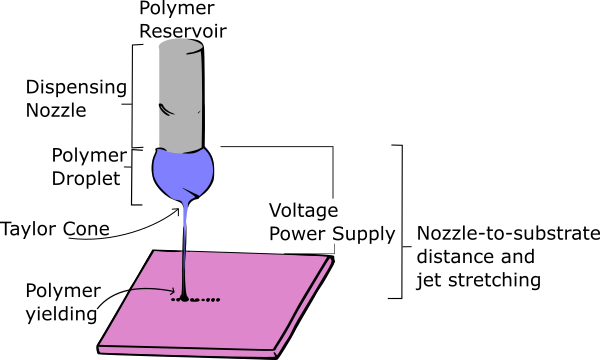
\includegraphics{images/43f61edd-73cd-4222-830e-3333f92934e9-uimg_nfesvariants.png}}{}
\makeatother 
\caption{{Near-Field ES Process Parameters}}
\label{f-3629d3a3f9cf}
\end{figure}
\egroup
To spin nano fibers at close distances, the initial diameter of the jet is required to be as small as possible since stretching of the thread is limited. Kameoka et al.\unskip~\cite{527120:12321556} demonstrated that a small initial spinning radius can be achieved using an atomic force microscope tip with a small polymer solution drop at the tip.

Near-field electrospinning, has exhibited to be capable fabricate nano fibers and nano fiber patterns \unskip~\cite{527120:11974321}. Nevertheless, having a small polymer solution drop at the nozzle tip limits the length of the fibers that can be fabricated in a continuous manner. Using a spinneret with a reservoir (e.g. syringe) of solution generally produces fibers with diameter of a few micrometers \unskip~\cite{527120:11974310,527120:11974326}, since it creates a limit to which the nozzle inner diameter can be reduced to allow the solution to flow through. As shown inFigure~\ref{f-51afaccaf109}, the implementation of thicker needle nozzles translate into an increase of the resulted fiber diameter

Coppola et al.\unskip~\cite{527120:11974307} have showed a NFES variant that allows polymer nano fibers to be deposited directly from a polymer drop, averting the issue of nozzle clogging. The fibers are also prone soaking after deposition thus giving the fibers a semi-circular cross-section as depicted in Xue et al.'s\unskip~\cite{527120:11974326} work.



\subsection{Nozzle spinneret}The thinnest nozzles in literature so far are about $50 nm $ in diameter, by Chang et al.\unskip~\cite{527120:11974306} who used a  $100 \mu m $ inner diameter needle tip to electrospin poly(ethylene oxide) (PEO). Camillo et al.\unskip~\cite{527120:12322072} used a micro-diameter tip Tungsten spinneret in a 26G needle to electrospin co-polymer, poly[2-methoxy-5-(2-ethylhexyloxy)-1,4-phenylenevinylene] (MEH-PPV) with poly(ethylene oxide) (PEO). The nozzle most commonly comprises a simple narrow-bore, blunt-end metal needle. The diameter of the needle can vary, but most commonly researches work with internal diameters below 1 $mm $ . This translates to needles of gauge 18{\textendash}22. In general, this simple spinneret design can be used to achieve successful spinning. A blunt-end rather than a tapered-end for the needle exit is important as the size distribution of the products increase with an increase in needle tip angle. However, it should be noted that there will be some interactions between the solvent and polymer molecules in the solution and the metal surface of the spinneret. There will exist some attractive forces between the polar groups in the polymer and the electro-positive metal surface, which can act counter to the drawing force of the electric field and can pull the polymer solution back into the spinneret. It has been found that coating the spinneret exterior in a non-conductive and non-stick polymer such as Teflon or epoxy coating can reduce these interactions.\unskip~\cite{527120:13082768,527120:13082811} As a result, the electrical energy can be more efficiently used to elongate and narrow the polymer jet, and narrower fibers can be produced. In addition, strong attractive forces between the polymer jet and the metal spinneret can result in fibers becoming attracted to the needle, leading to lower yields and potentially to blocking of the exit orifice.



\subsection{Applied Voltage}In recent literature, near field electrospinning has been studied to reduce the fiber diameter and to improve the fiber deposition accuracy. Madou et al.\unskip~\cite{527120:11973130} and Chang et al.\unskip~\cite{527120:11974306} came to the conclusion higher voltages yield thicker micro-fibers with a loss in jet stability. This relationship between the applied voltage and resulting fiber diameter is influenced by other variables such as nozzle-to-substrate distance and solution deposition rate. For instance, if a high voltage is applied at a low deposition rate then electrospraying is achieved, meaning the formation of several non-continuous fibers. The applied voltage shall be sufficient to break the surface tension and initiate the jet, but low enough to avoid multiple jets at the nozzle tip.

Madou et al.\unskip~\cite{527120:11973130} achieved the fabrication of thinner fibers with spatial control by reducing the applied voltage to 200-600 $V $  at a nozzle-to-substrate distance of 0.5-1 $mm $. The low voltage setting does not create enough charge to break the polymer solution surface tension to initiate the electrospinning process.

Madou et al.\unskip~\cite{527120:11973130} and Chang et al.\unskip~\cite{527120:11974306} initiated the electrospun fibers by mechanically pull the polymer solution at the nozzle tip using a micro-probe tip. Chang and coworkers reduced the applied voltage from 1.5 $kV $ to 600 $V $ with a nozzle-to-substrate distance of 500 $\mu m $ to yield a fiber diameter between 3 $\mu m $  and 50 $nm $ . With an applied voltage of 200 $V $ and a nozzle-to-substrate distance of 1 $mm $.

In near-field electrospinning, the applied voltage has an impact on the produced fiber morphology. For instance, a voltage higher or lower to the optimum voltage will translate into an increase in fiber diameter. Song et al.\unskip~\cite{527120:11974320} demonstrated that a decrease in voltage from 400 to 500 $V $ can reduce the fiber diameter from 160 to about 60 $nm $with a nozzle-to-substrate distance of 20 $\mu m $. A workaround to break the polymer solution surface tension is to initialize the NFES process with a higher voltage and then lower the voltage once the jet is created. Huang et al.\unskip~\cite{527120:11974311} implemented the previous and yield ordered fibers with a distance between adjacent fibers of 50 $\mu m $.



\subsection{Nozzle-to-substrate distance}
\bgroup
\fixFloatSize{images/4cc65220-1457-4d0d-bb04-9b1c8138aa96-uffes_vs_nfes.png}
\begin{figure*}[!htbp]
\centering \makeatletter\IfFileExists{images/4cc65220-1457-4d0d-bb04-9b1c8138aa96-uffes_vs_nfes.png}{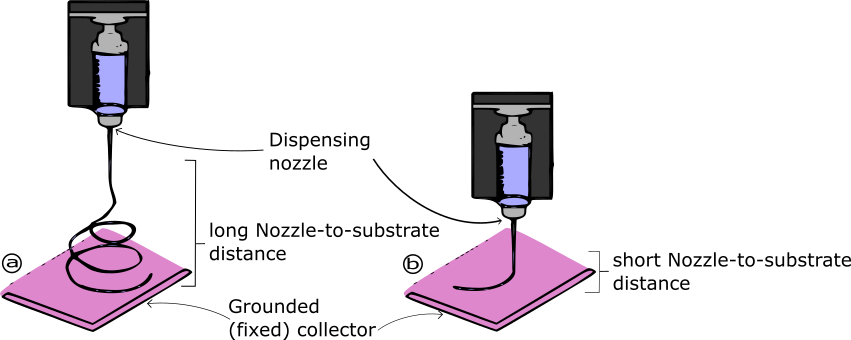
\includegraphics{images/4cc65220-1457-4d0d-bb04-9b1c8138aa96-uffes_vs_nfes.png}}{}
\makeatother 
\caption{{a) Typical Far-field Electrospinning (FFES) Setup. b) Typical Near-field Electrospinning (NFES) Setup.}}
\label{f-c34559531e3e}
\end{figure*}
\egroup
Figure~\ref{f-c34559531e3e}.a, depicts the typical setup for the conventional far-field electrospinning (FFES). As stated in previous sections, the precursor polymer droplet becomes charged with the employment of an electric field between the polymer solution and the collector\unskip~\cite{527120:14135125}. When the polymer solution surface tension is overcome by the electric field potential difference a jet is formed, starting the electrospinning process. The electrospinning process can be break down into two steps: i) first the jet travels in a straight line, and ii) the jet begins to curl due to bending and whipping instabilities \unskip~\cite{527120:13444381,527120:14135543}. The fiber spatial control in far-field electrospinning is limited due to the instabilities, inhibiting the precise deposition of fibers.

In the intent to achieve controlled fiber deposition, Sun et al. \unskip~\cite{527120:11974321} reported an electrospinning variation known as near-field electrospinning (NFES),Figure~\ref{f-c34559531e3e}.b, describes the near-field electrospinning setup, where the distance between the dispensing nozzle and the collector is reduced to write fibers while the jet travels in a straight line. Moreover, some mechanical influence is required to deposit fibers precisely. The mechanical force is introduced by moving collector. If the polymer solution jet speed is faster than the speed of the moving collector, the written fiber will curl; on the other hand, if the collector moves faster than the polymer jet, the fiber will gradually diminish \unskip~\cite{527120:11974327,527120:11974326}. Currently, due to the lack of theoretical models, the near-field electrospinning process parameters (such as the collector speed) are typically tuned by experience and experimentation only.

The main difference between NFES and FFES is the distance between the needle and the collector which is higher in FFES (about 10 cm) compared to NFES which ranges in the mm scale. The short distance allow the production of well aligned fibers within particular designs. In NFES, the fiber morphology can be altered by the control of the distance between the nozzle and the substrate (collector). With the decrease of the nozzle-to-substrate distance, the electric field strength increases; however it can cause incomplete solvent volatilisation and possible short circuits between the collector and the nozzle tip.

An optimal nozzle-to-substrate distance shall be defined to ensure the fabrication of dry continuous fibers. If the solvent is not well evaporated, the produced fibers are prone to defects; on the other hand if solidification happens too fast, the solids can block the spinneret which can prevent a continuous fiber yield. Furthermore, the polymer jet will discharge itself as soon as possible, therefore long distances can result in low yields.



\subsection{Substrate}Due to the close distance between the grounded substrate and the charged spinneret in NFES, the set up is prone to electrical shorts. In NFES, when a short circuit takes place, the electrospinning process is interrupted resulting in the fabrication of discontinuous fibers. Two workarounds to avoid electrical shorts is to lower the applied voltage and to use less conductive substrates \unskip~\cite{527120:11974315,527120:12322289}.

Liu et al.\unskip~\cite{527120:11974315} discovered that the fiber alignment is improved by using a glass-cooper foil substrate, however the well aligned fibers are spoiled after prolonged depositions due to residual charges. Additionally, the effect of residual charges is amplified with the used collector substrate contains a conductive layer and a non-conductive layer\unskip~\cite{527120:11974315}.

On the other hand, Choi et al.\unskip~\cite{527120:12322289} implemented a hydrophilic substrate to deposit the fibers with plasma treatment to increase the conductivity of selected areas. NFES was carried put with precise deposition as the fibers were placed as per the desired design within the hydrophilic substrate.
    
\section{Discussion \& NFES Challenges}
Helix electrodynamic printing (HE-printing) was presented by Duan et al. \unskip~\cite{527120:11974308} with the intention of depositing aligned fibers. The authors fabricated a stretchable piezoelectric device using micro and nano fibers to demonstrate the possible applications of HE-printinh for electronics manufacturing. Duan et al. concluded that the fiber morphology is mainly driven by: the stage velocity, the applied voltage, and the nozzle-to-collector distance.


\bgroup
\fixFloatSize{images/6e169654-19e4-40ab-bb05-8ffb11b5ce11-uplt_cormat.png}
\begin{figure*}[!htbp]
\centering \makeatletter\IfFileExists{images/6e169654-19e4-40ab-bb05-8ffb11b5ce11-uplt_cormat.png}{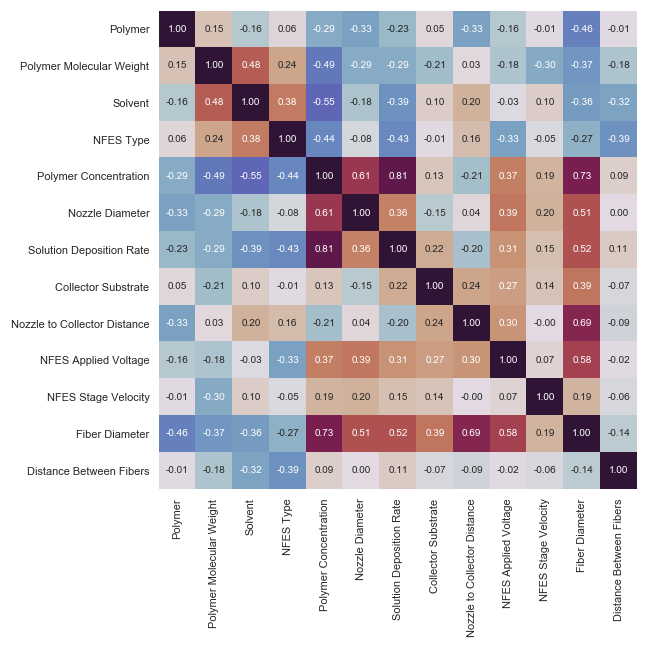
\includegraphics{images/6e169654-19e4-40ab-bb05-8ffb11b5ce11-uplt_cormat.png}}{}
\makeatother 
\caption{{}}
\label{f-30543905e028}
\end{figure*}
\egroup

\bgroup
\fixFloatSize{images/dac8d1ee-e40f-49ab-a2ca-e0d7db210474-uplt_nfesappliedvoltage_vs_fiberdiameter.png}
\begin{figure*}[!htbp]
\centering \makeatletter\IfFileExists{images/dac8d1ee-e40f-49ab-a2ca-e0d7db210474-uplt_nfesappliedvoltage_vs_fiberdiameter.png}{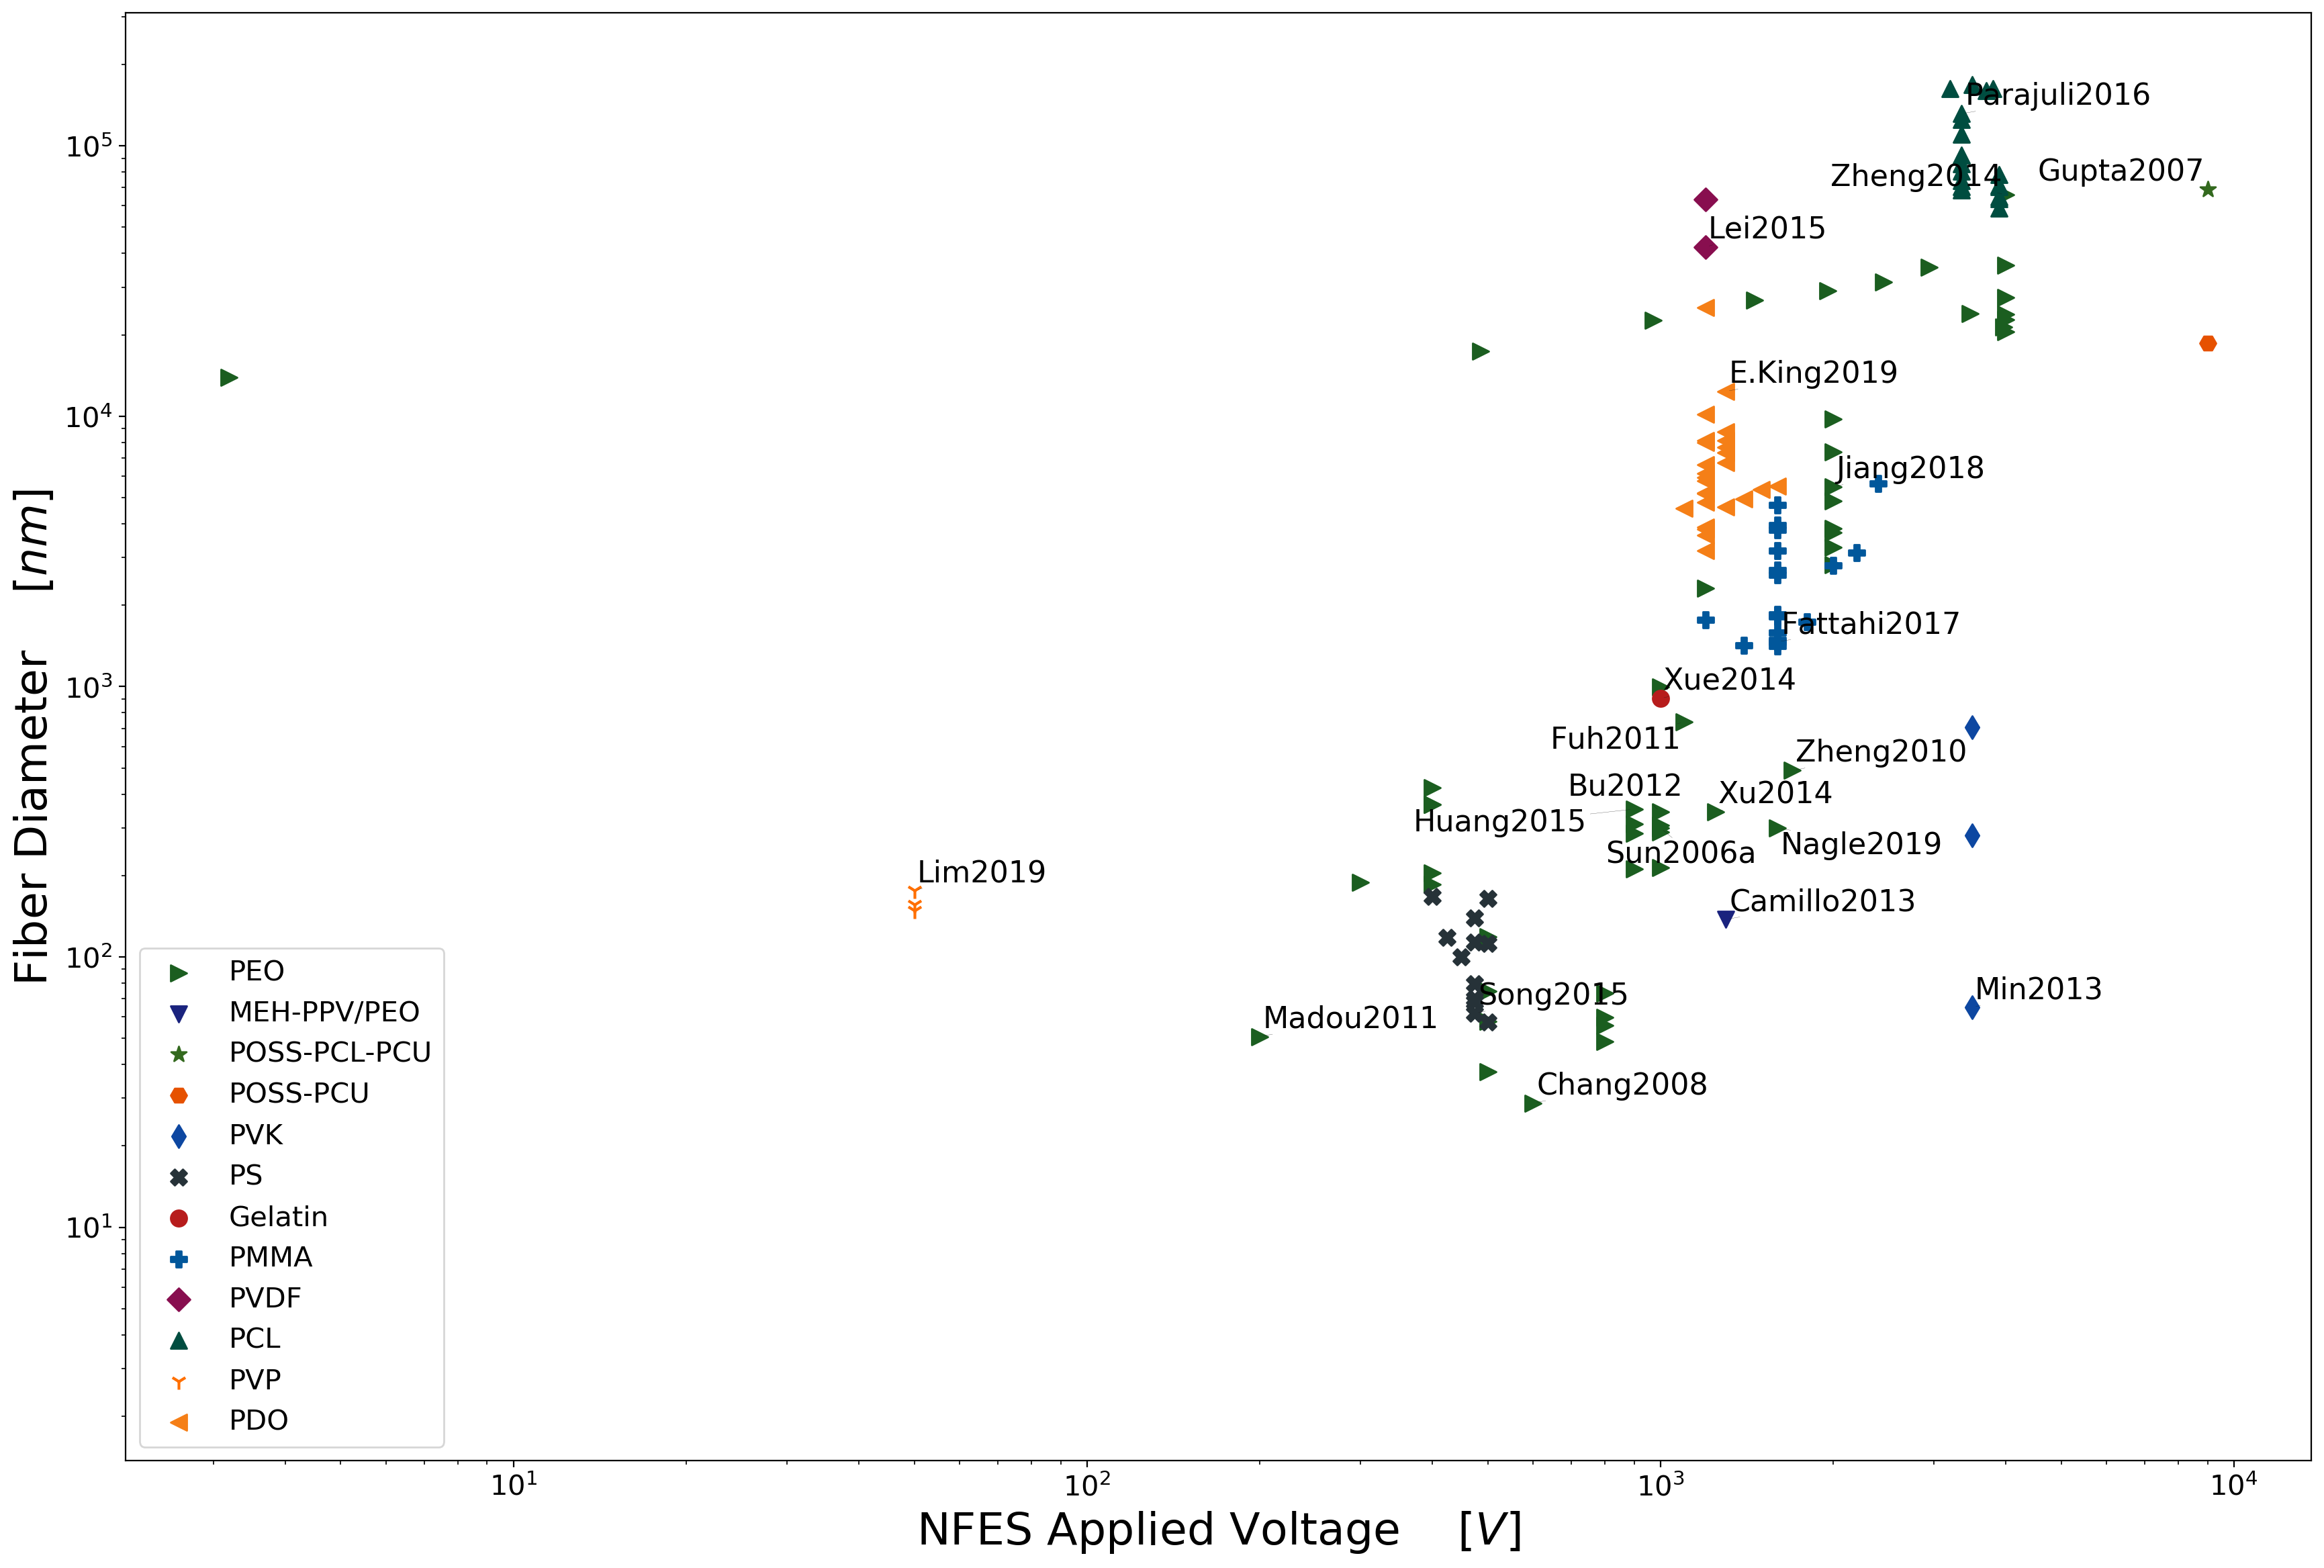
\includegraphics{images/dac8d1ee-e40f-49ab-a2ca-e0d7db210474-uplt_nfesappliedvoltage_vs_fiberdiameter.png}}{}
\makeatother 
\caption{{NFES Applied Voltage vs. Fiber Diameter}}
\label{f-59ed68f95344}
\end{figure*}
\egroup

\bgroup
\fixFloatSize{images/a8f86e3c-c4e3-45be-b9e8-7b60145137cb-uplt_nozzlediameter_vs_fiberdiameter.png}
\begin{figure*}[!htbp]
\centering \makeatletter\IfFileExists{images/a8f86e3c-c4e3-45be-b9e8-7b60145137cb-uplt_nozzlediameter_vs_fiberdiameter.png}{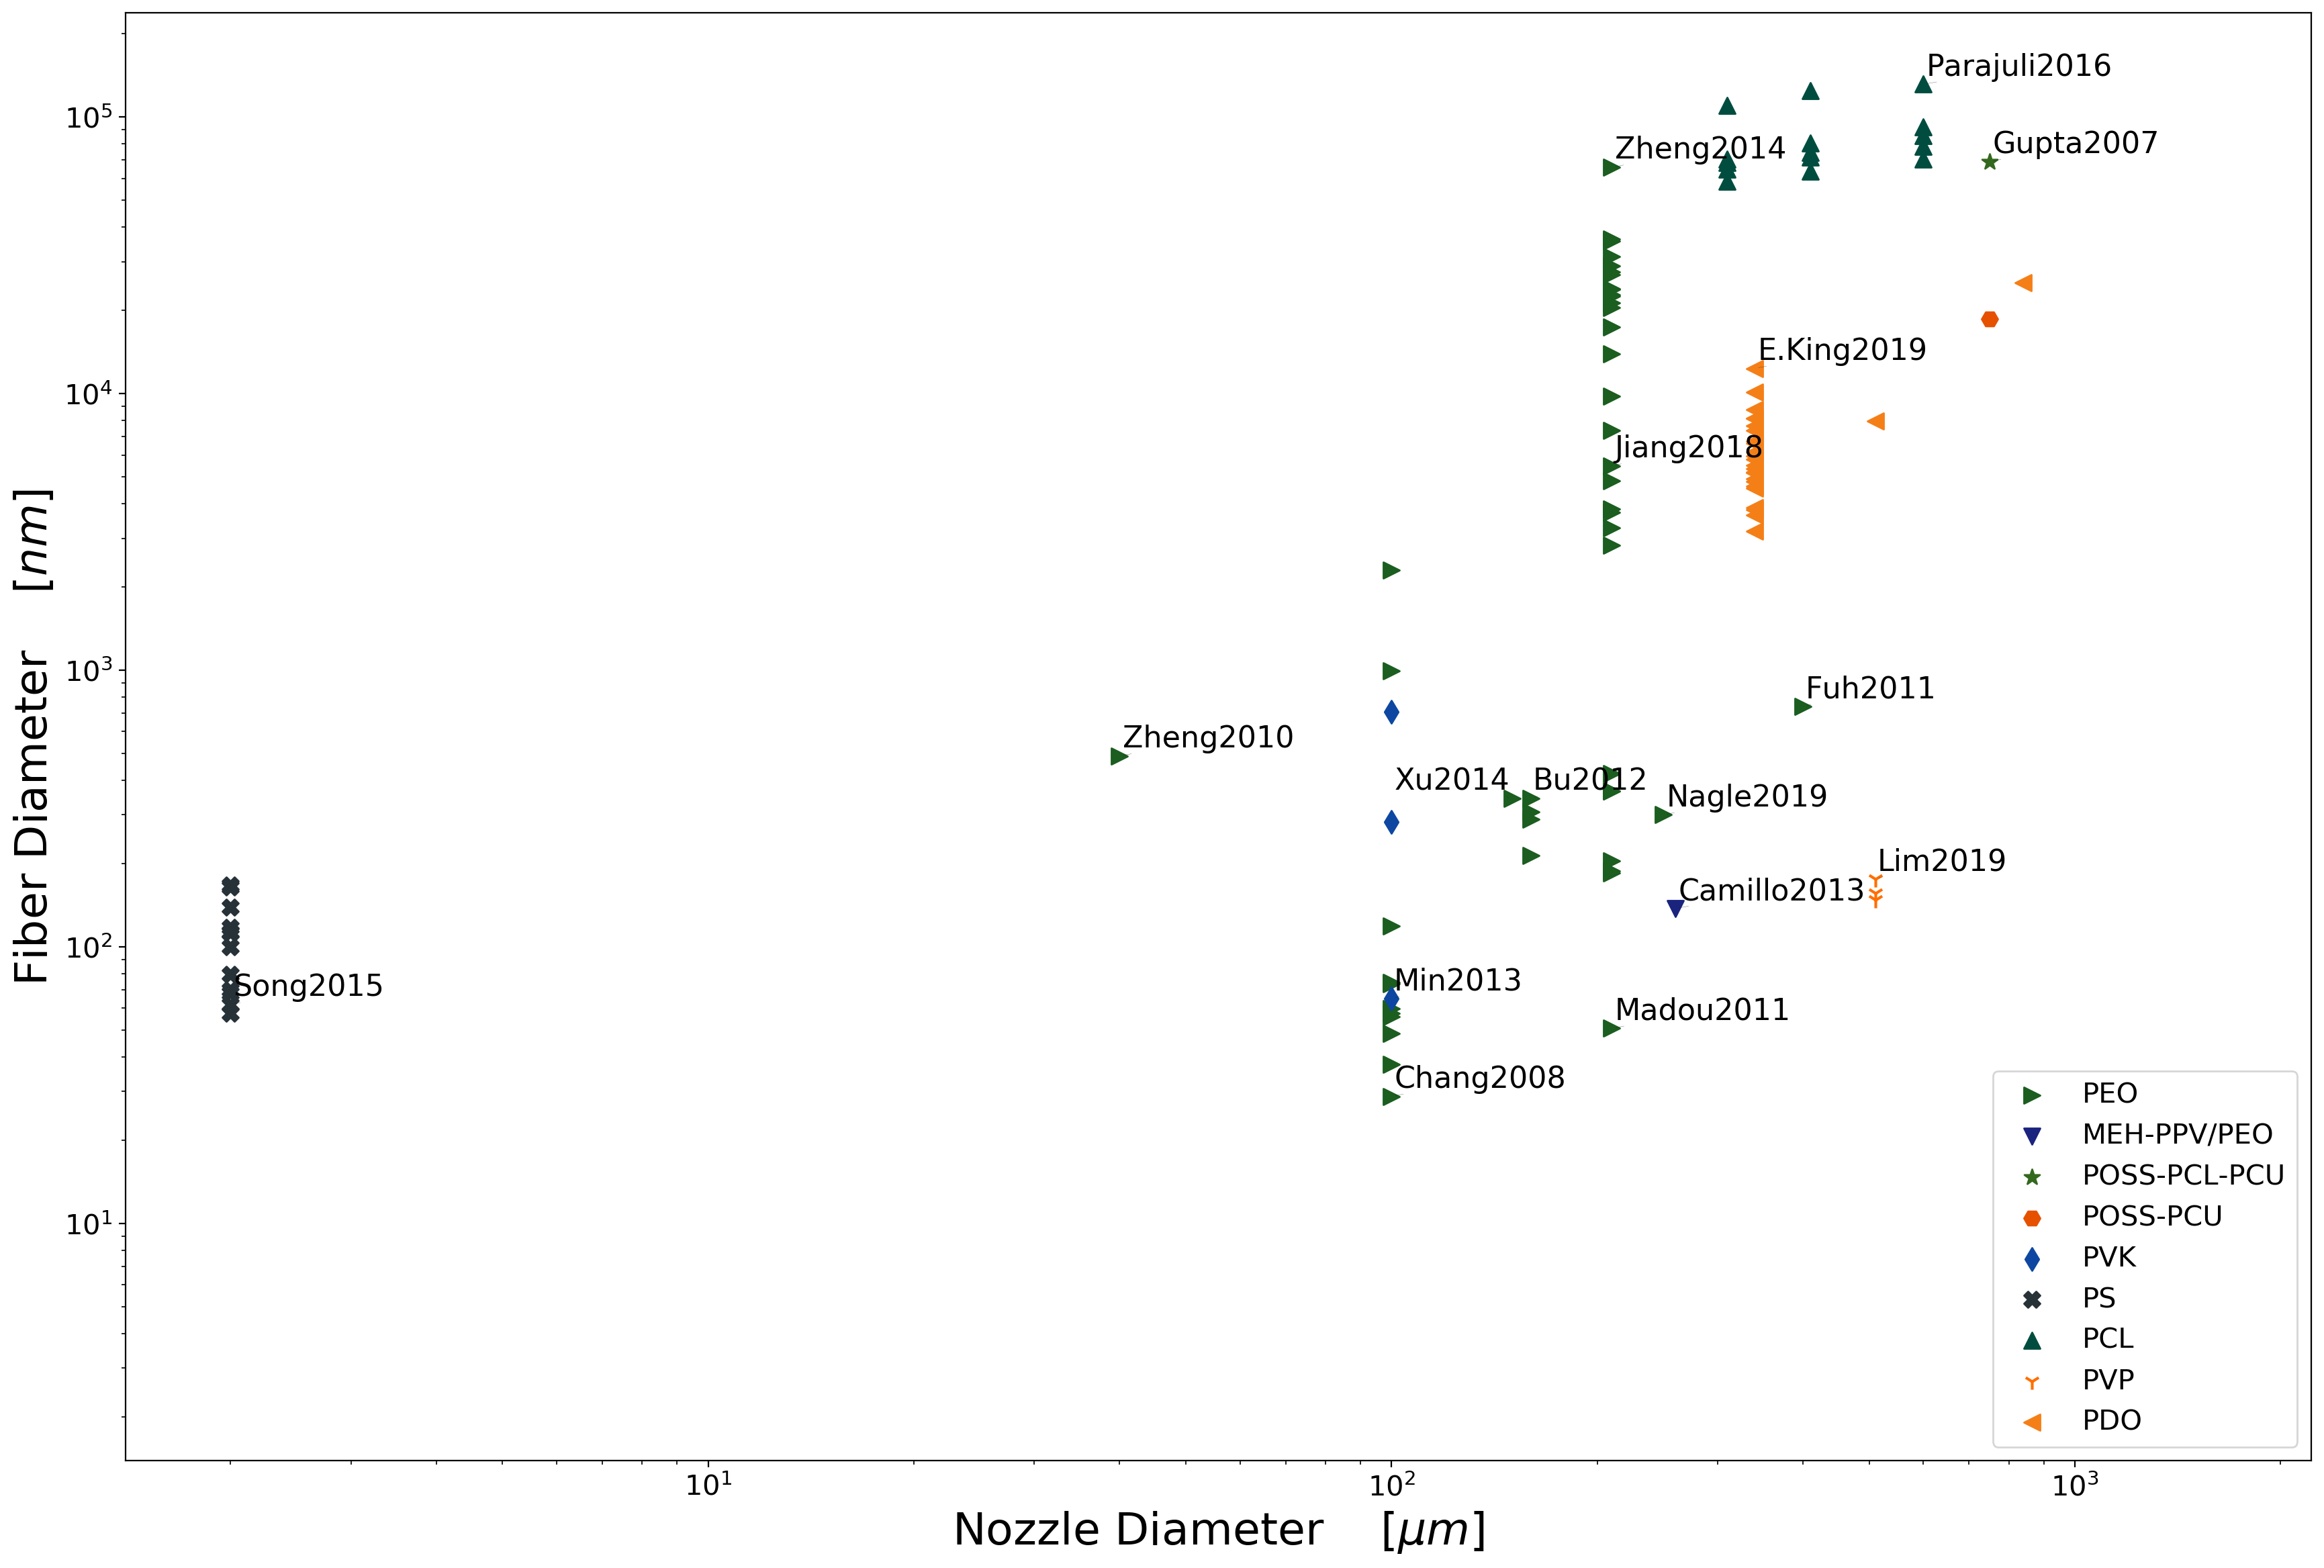
\includegraphics{images/a8f86e3c-c4e3-45be-b9e8-7b60145137cb-uplt_nozzlediameter_vs_fiberdiameter.png}}{}
\makeatother 
\caption{{Nozzle Diameter vs. Fiber Diameter}}
\label{f-51afaccaf109}
\end{figure*}
\egroup

\bgroup
\fixFloatSize{images/6eaa2ba7-07ab-4cfb-980d-5f78b4fcf1a5-uplt_nozzletocollectordistance_vs_fiberdiameter.png}
\begin{figure*}[!htbp]
\centering \makeatletter\IfFileExists{images/6eaa2ba7-07ab-4cfb-980d-5f78b4fcf1a5-uplt_nozzletocollectordistance_vs_fiberdiameter.png}{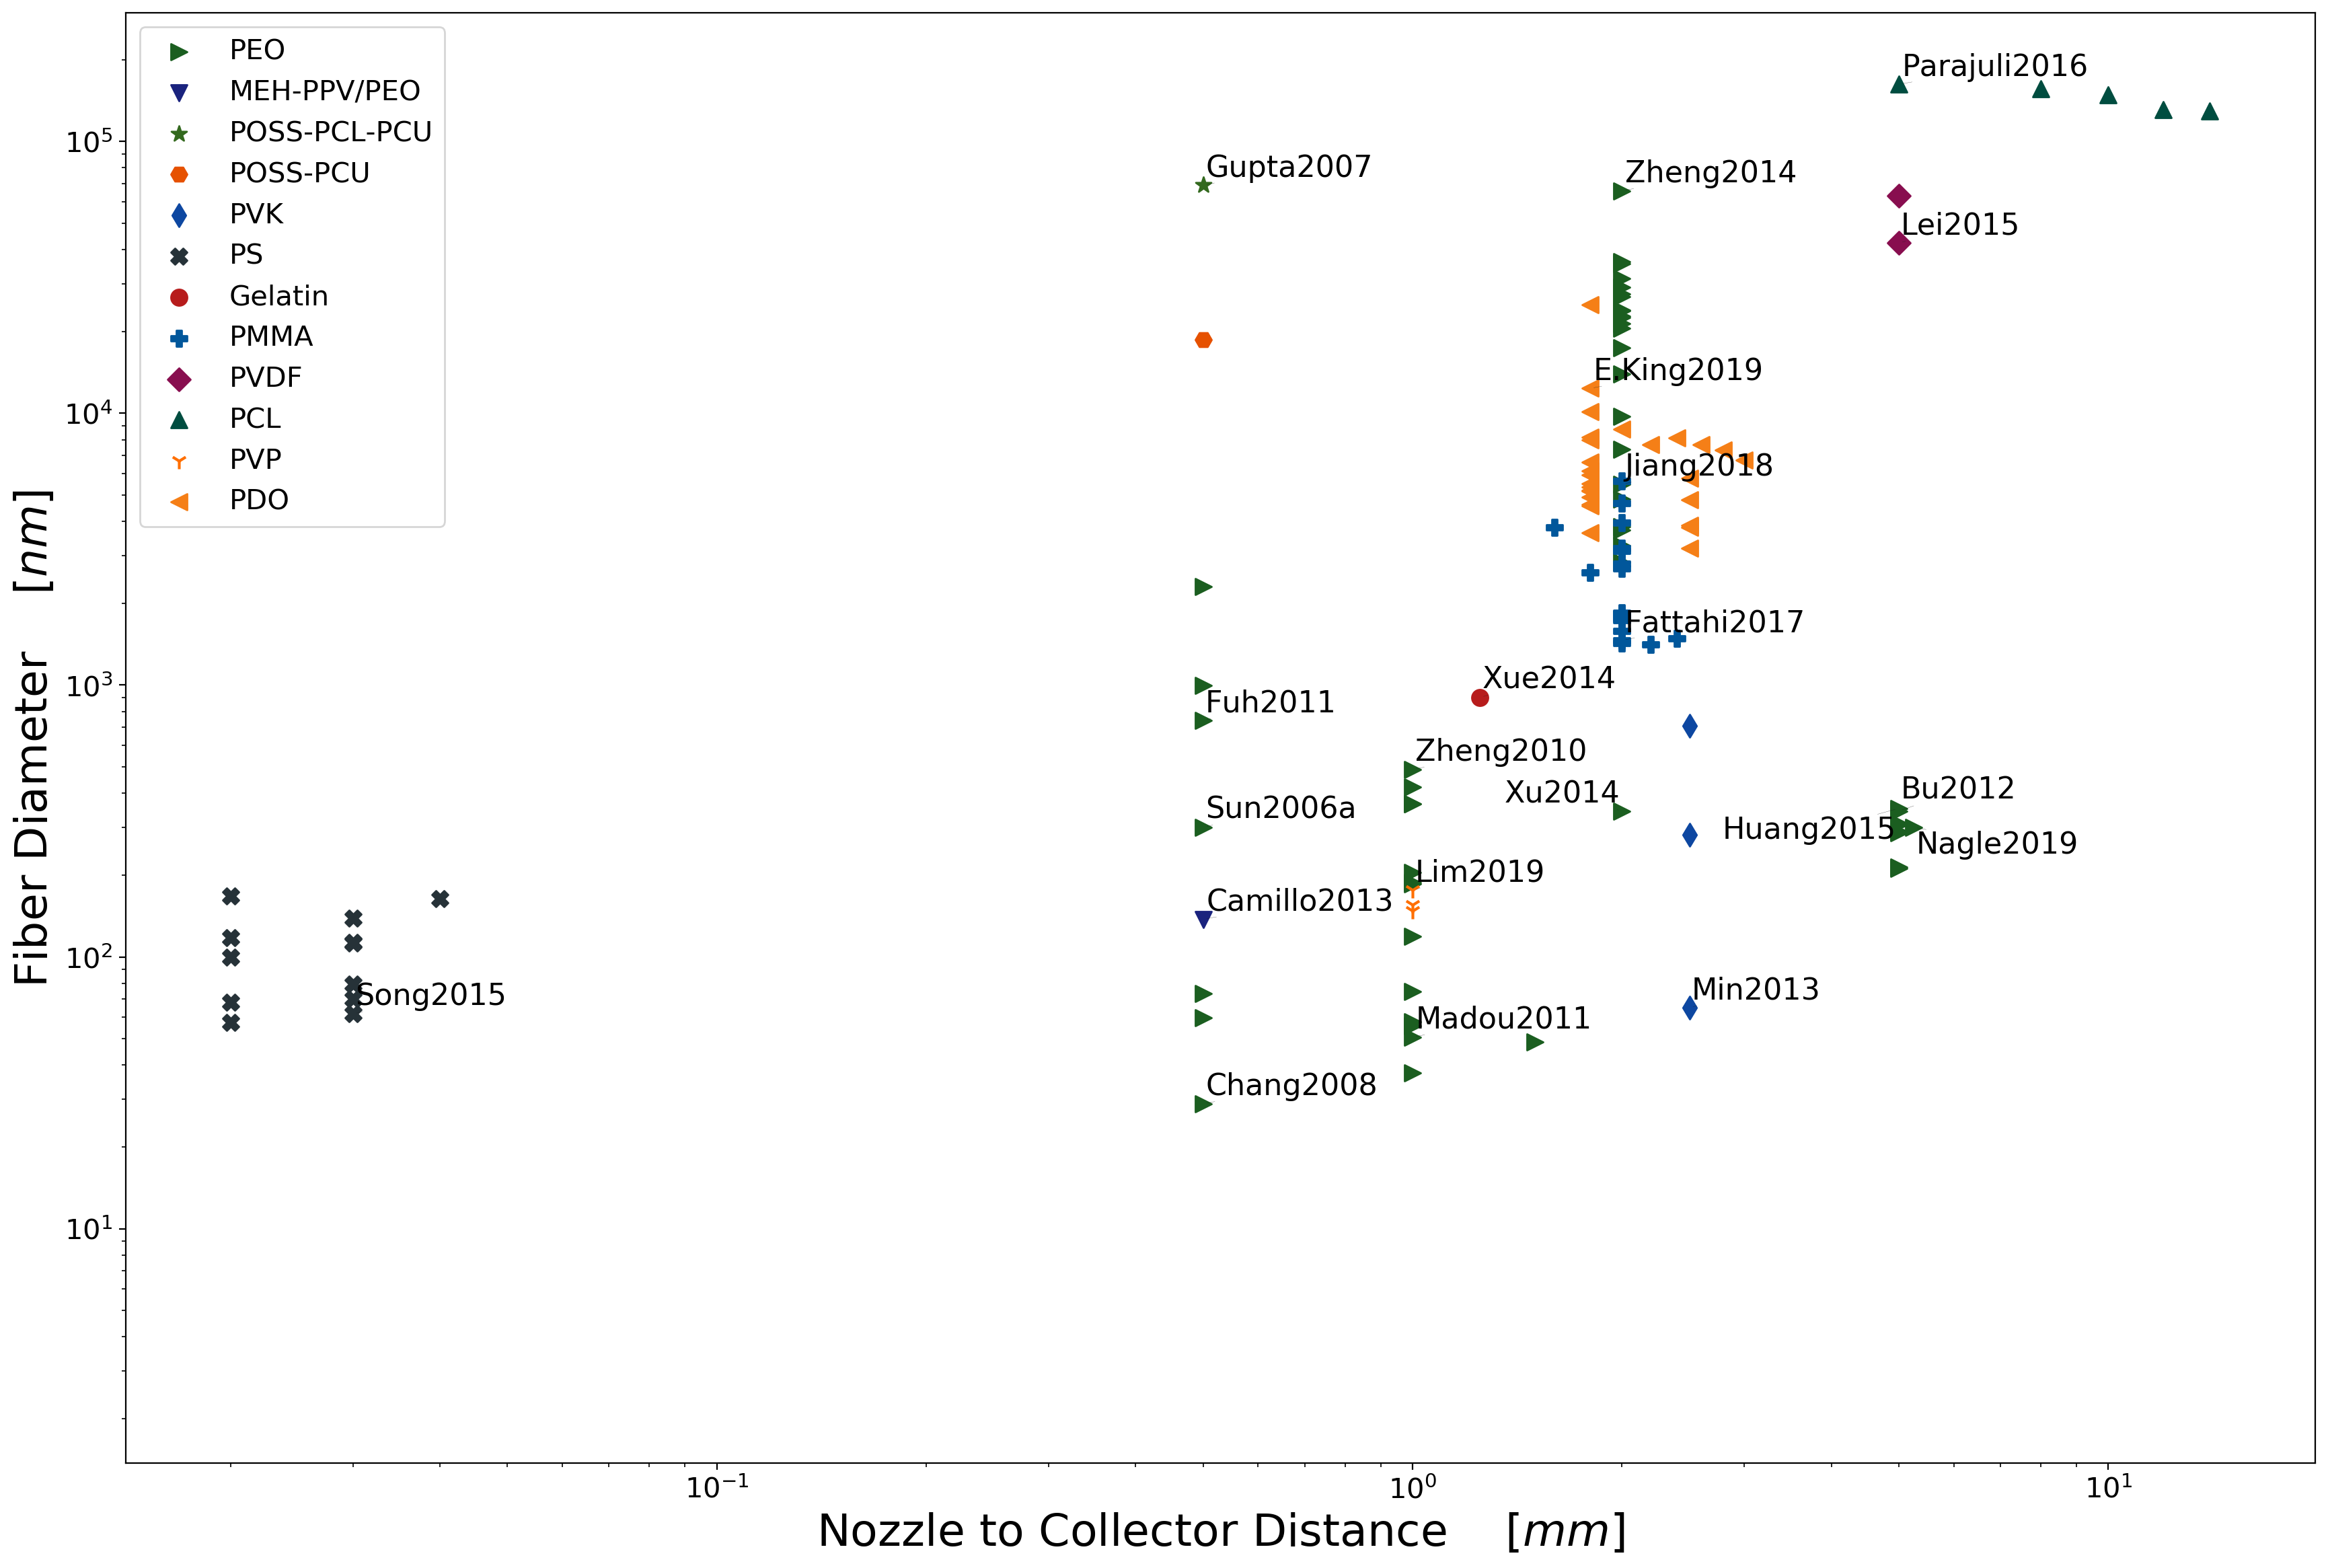
\includegraphics{images/6eaa2ba7-07ab-4cfb-980d-5f78b4fcf1a5-uplt_nozzletocollectordistance_vs_fiberdiameter.png}}{}
\makeatother 
\caption{{Nozzle to Collector Distance vs. Fiber Diameter}}
\label{f-5f453fad619f}
\end{figure*}
\egroup

\bgroup
\fixFloatSize{images/b8cbc9c7-97d8-409f-a979-447aebd4aa67-uplt_polymerconcentration_vs_fiberdiameter.png}
\begin{figure*}[!htbp]
\centering \makeatletter\IfFileExists{images/b8cbc9c7-97d8-409f-a979-447aebd4aa67-uplt_polymerconcentration_vs_fiberdiameter.png}{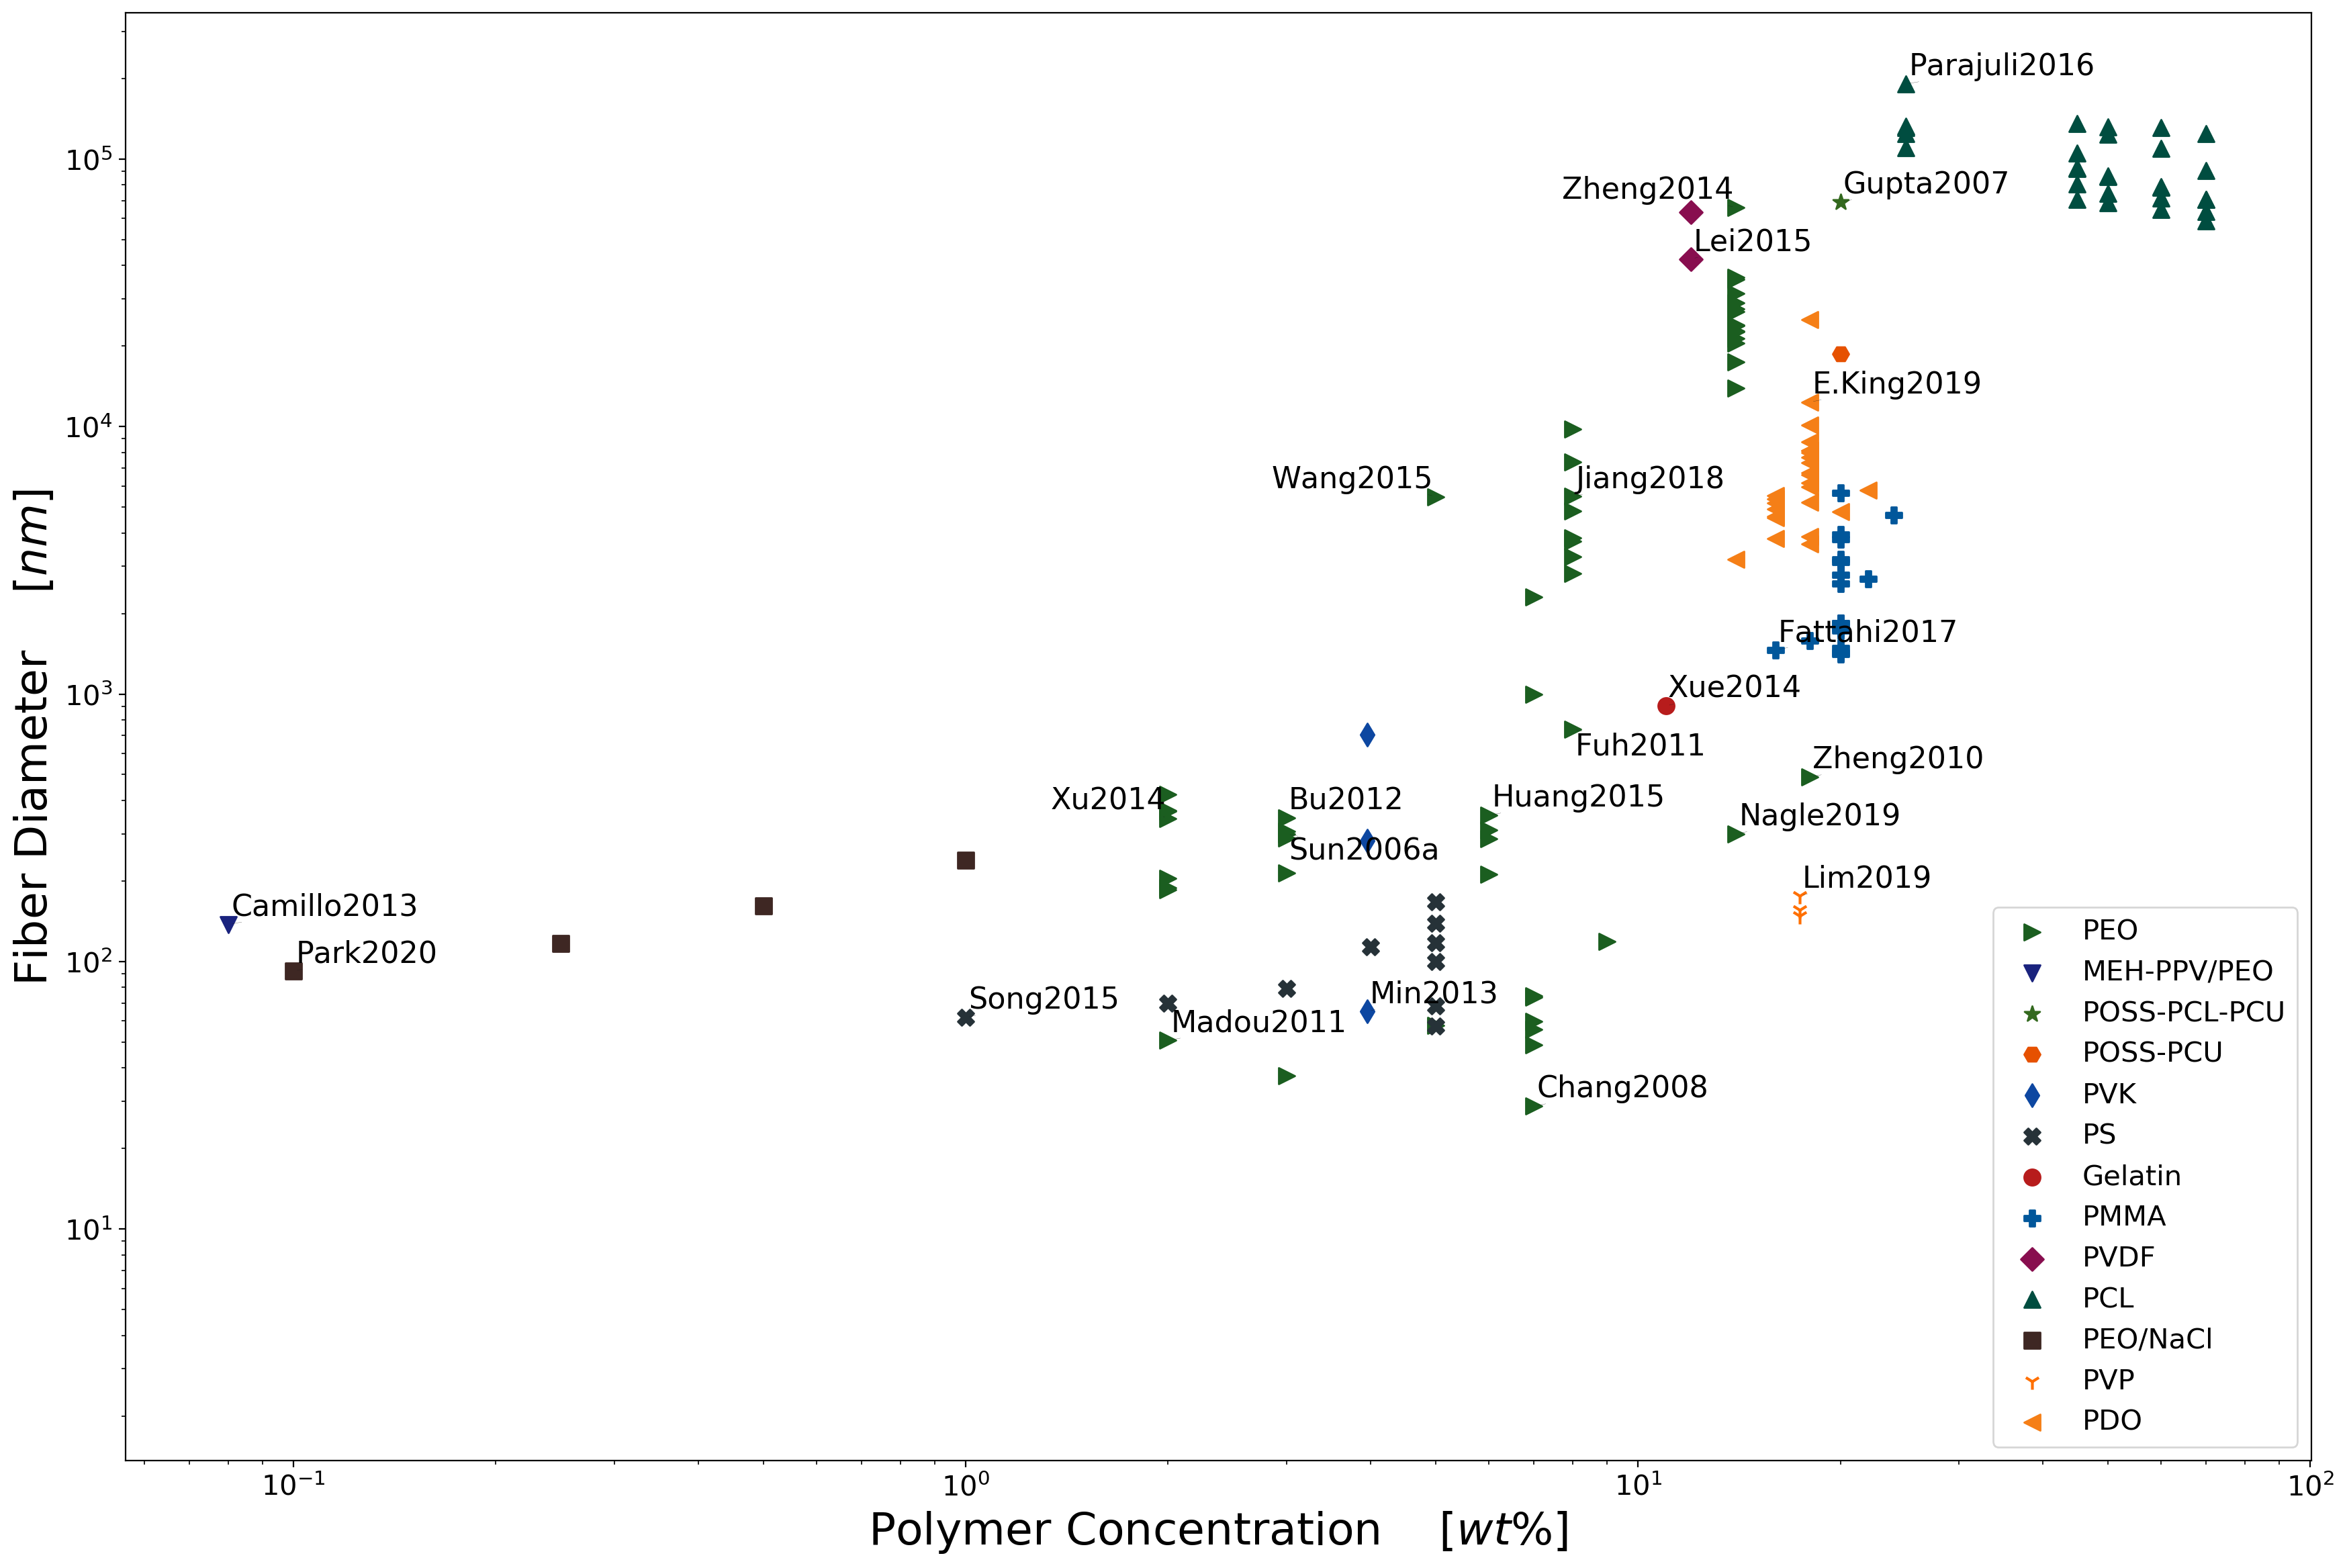
\includegraphics{images/b8cbc9c7-97d8-409f-a979-447aebd4aa67-uplt_polymerconcentration_vs_fiberdiameter.png}}{}
\makeatother 
\caption{{Polymer Concentration vs. Fiber Diameter}}
\label{f-d977f56a0782}
\end{figure*}
\egroup

\bgroup
\fixFloatSize{images/085b1fe7-0896-4800-b231-bf68cf86983b-uplt_solutiondepositionrate_vs_fiberdiameter.png}
\begin{figure*}[!htbp]
\centering \makeatletter\IfFileExists{images/085b1fe7-0896-4800-b231-bf68cf86983b-uplt_solutiondepositionrate_vs_fiberdiameter.png}{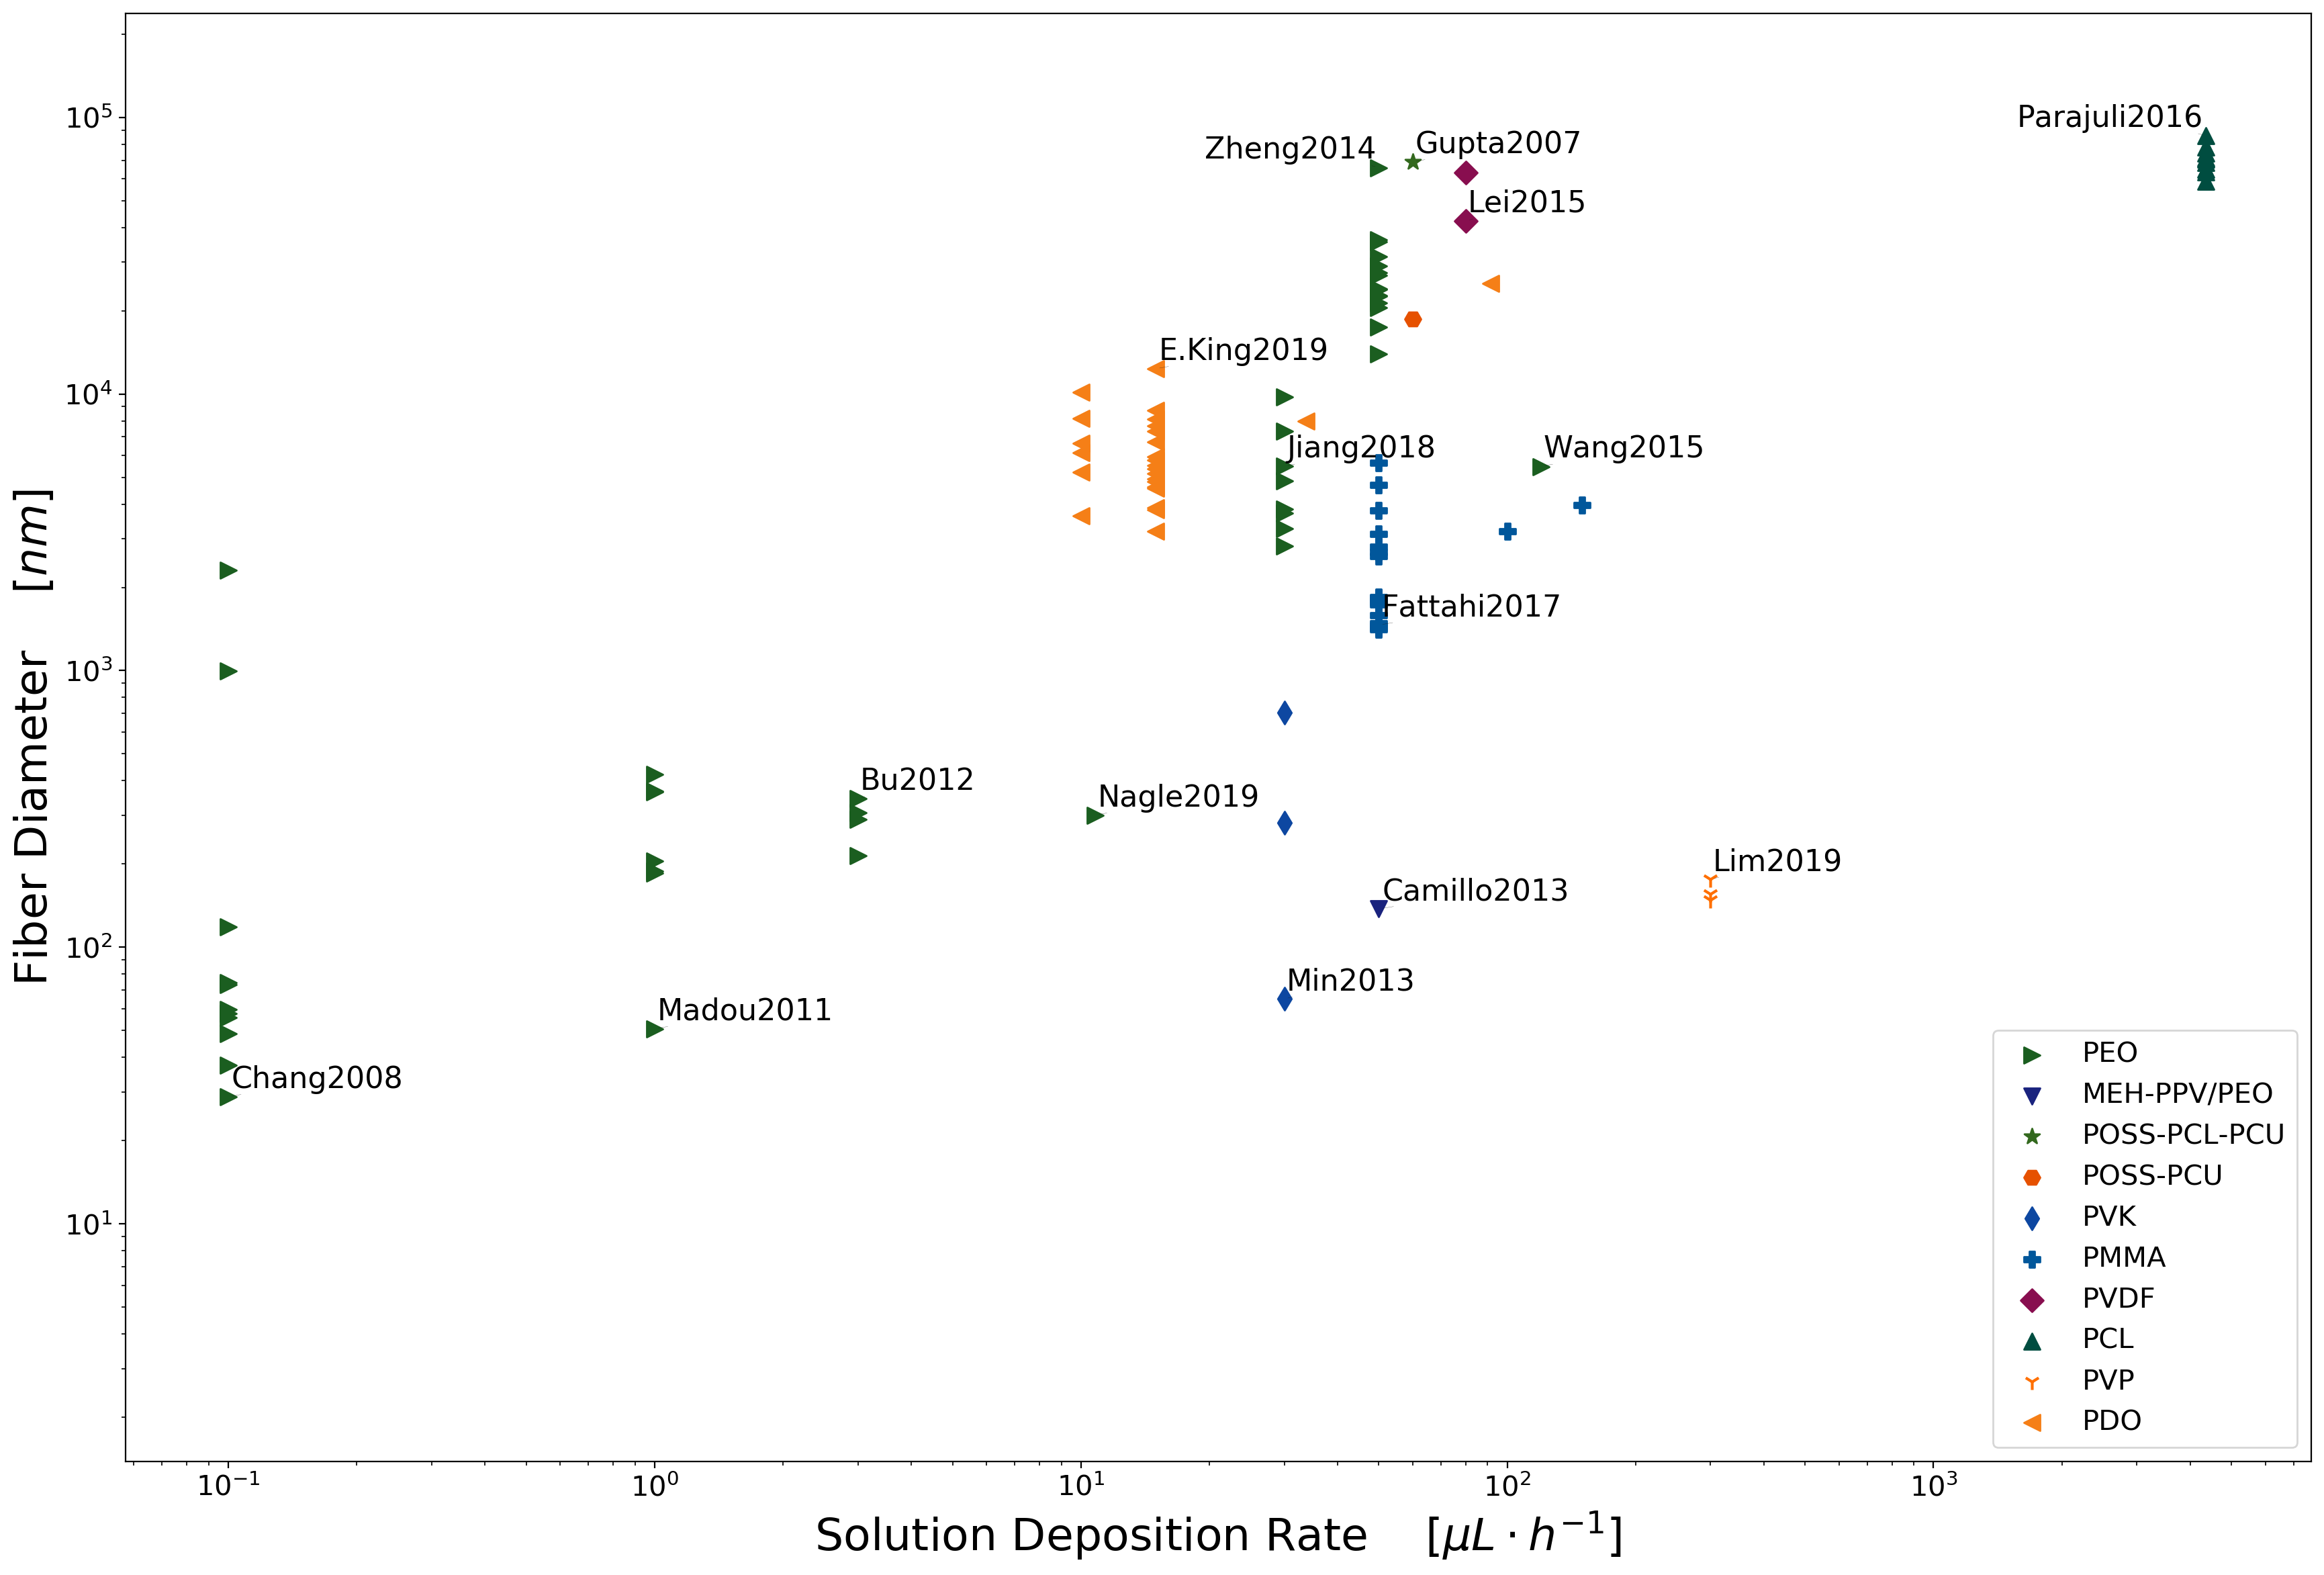
\includegraphics{images/085b1fe7-0896-4800-b231-bf68cf86983b-uplt_solutiondepositionrate_vs_fiberdiameter.png}}{}
\makeatother 
\caption{{Solution Deposition Rate vs. Fiber Diameter}}
\label{f-08e527ddef81}
\end{figure*}
\egroup
Electrohydrodynamic (EHD) jet printing is a direct-writing technique which ejects ink through a fine nozzle using an electric field, which has the advantages of high-resolution, rapid printing speed and a wide range of ink selectivity. The effect of parameters such as ink concentration, working distance, applied voltage, and stage speed on the diameter of the printed nano fibers was investigated.

Near-field electrospinning (NFES) is widely recognized as a versatile nano fabrication method, one suitable for applications in tissue engineering. Rapid developments in this field have given rise to layered nano fibrous scaffolds. However, this electrostatic fabrication process is limited by the electric field inhibitory effects of polymer deposition. This leads to a major challenge: how to surpass this limitation on planar/layered constructs. While the current focus in this area largely lies with the investigation of new materials, techniques and increasing precision of NFES systems and patterning, exploration of complex collector substrates is often restricted by (i) available technology and (ii) access to complex electrode manufacturing tools.

Although electrospinning (ES) allows the production of unsurpassed nano scale polymer fibers, the major drawbacks are the nozzle-clogging and single-jet spinneret, respectively. This is a real limitation in terms of usable polymers and for patterning active organics. Nowadays the micro-engineering of smart materials could represent a new route for many fields of technology ranging from the production of electronic and photonic devices [1\ensuremath{-}3] to regenerative medicine and tissue engineering. [4\ensuremath{-}7] An enormous technological interest is related to the possibility of patterning fibers directly in well-ordered patterns avoiding the deposition of nonwoven sub micrometer mats often occurring in ES. [8,9] In the past decade several attempts have been made using field- induced [10\ensuremath{-}13] and near-field ES, [14,15] but only very recently, with the introduction of mechano ES, [16] has the production of well- ordered fiber patterns been achieved. Nevertheless, some drawbacks related to the complexity of the setup, the operating temperature, and the selection of usable materials for problems related to nozzle clogging still persist. Moreover, high temperature can cause deterioration of the optical and electronic properties of active organic materials eventually embedded in the functionalize [d fibers. On the other side, interfering effects due to closeness of multiple electrified nozzles ban working with multiple spinnerets.
\apptocmd{\thebibliography}{\csname phantomsection\endcsname\addcontentsline{toc}{section}{\numberline{}\refname}}{}{}
    



\bibliographystyle{elsarticle-num}

\bibliography{\jobname}

\end{document}
